\documentclass{article}

\usepackage{amsmath,amsthm,amsfonts,amssymb,bm}
\addtolength{\textheight}{5.0cm}
\addtolength{\voffset}{-3.5cm}
\addtolength{\hoffset}{-2.5cm}
\addtolength{\textwidth}{5.0cm}

\allowdisplaybreaks

\usepackage{subeqnarray}
\usepackage{mathrsfs}
\usepackage[usenames,dvipsnames]{color}
\usepackage{url}
\usepackage{ulem}
\usepackage{indentfirst}
%\usepackage{textcomp}
%\usepackage{graphics}
\usepackage{graphicx}
\usepackage[hang,small,bf]{caption}
\setlength{\captionmargin}{50pt}

%includeonly{}


\graphicspath{{Figures/}{Figures/CPL/}{Figures/DE/}{Figures/P/}}


%\usepackage{tikz}
%\usetikzlibrary{mindmap,trees}

\begin{document}
\title{Power Spctrum \& Its Evolution}
\author{MA Lei}
\maketitle


%%%%Inclule thse files please.%%%




%%%%%%%%%%%%%%%%%%%%%%%%%%%%%%%%%%%%%%%%%%%%%%
%%%%%%%%%%%%%%%%%%%%%%%%%%%%%%%%%%%%%%%%%%%%%%
%%%%%%%%%%%%%%%%%%%%%%%%%%%%%%%%%%%%%%%%%%%%%%
%%%%%%%%%%%%%%%%%%%%%%%%%%%%%%%%%%%%%%%%%%%%%%
%%%%%%%%%%%%%%%%%%%%%%%%%%%%%%%%%%%%%%%%%%%%%%
%%%%%%%%%%%%%%%%%%%%%%%%%%%%%%%%%%%%%%%%%%%%%%
%%%%%%%%%%%%%%%%%%%%%%%%%%%%%%%%%%%%%%%%%%%%%%




\hrule\vspace{1pt}\hrule
\begin{center}
\mbox{{\bf Harrison Zeldovich Prescription}} \\
\vspace{0.5em}
\mbox{{Harrison(1970) \& Zeldovich(1972)}}
\end{center}
\hrule



\section{Harrison Zeldovich Prescription}
All perturbations that come into the horizon have the same amplitude.
\begin{equation}
\Delta(k_i,t_i)=\Delta(k_e,t_e)=\text{Const.} \label{HZP}
\end{equation}

\paragraph{Attention} $k=2\pi/L$ is the comoving wavenumber.







\subsection{What does that mean? \& Evolution of This Prescription.}

One kind of understanding of the assumption is
\begin{enumerate}
\item
The perturbations are generated to be the same value (comoving value).

\item
When the perturbations are outside of the horizon, their comoving measurement do not evolve.

\end{enumerate}

However, this might be wrong (and it is wrong
%footnote
\footnote{Even the largest scale potential perturbations damp to $9/10$ of their original value.}
%END footnote
). This only gives us a intuitive inspiration. The only thing we know is \ref{HZP}.



\vspace{2ex}
\begin{quote}


{\bf{Am I wrong?}}

The assumption firstly used is $\delta_0=\beta_E N^{-n}$. Or equivalently, $\delta_0\propto L^{-3n}$. Since Harrison proved that there is a throshold epoch where the initial perturbations are located, all the perturbations generated at that epoch can be discribed as $\delta_0\sim L^{-3n} \sim k^{3n}$ and $n=\frac{2}{3}$. i.e., primiordial perturbations are $\delta_0\sim L_0^{-2}\sim a(t_H)^2/L_{H-physical}^2$. [$t_0$ denotes the time when the perturbation are generated. $t_H$ is the time of horizon crossing, i.e., $2ct_H=\lambda_H$.]

\begin{quote}


During RD, $a(t)^2=2\sqrt C t$, then $\delta_H\sim a(t_H)^2/t_H^2 \sim a(t_H)^2/a(t_H)^4 \sim 1/t_H$. The amplitude of the perturbations are time dependent because the moment of horizon crossing $t_H$ are different for different perturbations. So what are the mistakes here?
\end{quote}


If $\delta_H\sim k_H^2$ remains the same for all perturbations and $P(k_H)\sim k_H$, from the defination of another measurement of perturbations
\begin{equation}\Delta(k)=\frac{k^3}{2\pi^2}P(k),
\end{equation}
we have $\Delta^2=\delta_H^2$ when the perturbation comes into the horizon ($k=\lambda_H$), which indicates \ref{HZP}.

Generally speaking, one would choose the initial power spectrum to be power law form, i.e., $P(k)\propto k^n$, or evern more simple, scale free Zeldovich spectrum, $P(k)\propto k$.
%%%%%%%%%%   Footnote     %%%%%%%%%%%
\footnote{\begin{url} {http://fisica.usac.edu.gt/public/curccaf_proc/borganihtml/node5.html}
\end{url}
}
%%%%%%%%%%%%%%%%%%%%%%%%%%%%%%%%%%
 
\end{quote}


\subsubsection{Primitive Spectrum}
It is expected that $\Delta$ is scale free.
The primitive spectrum given by inflation (or just a dimension analysis) is
\begin{equation}
P_\Phi(k)=\frac{50\pi^2}{9k^3}\bigg( \frac{k}{H_0} \bigg)^{\hat{n}-1}\delta_H^2\bigg(\frac{\Omega_m}{D_1(a=1)}\bigg)^2
\end{equation}

When $\hat{n}=1$, that is exact a scale invariant perturbation, i.e., $P(k)\sim k^{-3}$


\begin{quote}
THE PROBLEM IS, How do the orginal $\mu_0\sim L_0^{-3n}\sim k_0^2$ evolve to $P(k_0)\sim k_0$?
\begin{eqnarray}
P(k_0)\sim \mu_0^2/k_0^3 \sim k_0.
\end{eqnarray}
\end{quote}




















\iffalse


%%%%%%%%%        #Harrison(1970)#          %%%%%%%%%%%%%%
\section{Harrison(1970)}


%%%%%%%%%%    ##Notations##     %%%%%%%%%%%%%

\setcounter{section}{0}


\subsection{Notations} 

\begin{quote}
0 subscript denotes the initial value \\
* subscript denotes the threshold value \\
$\mu=\delta\rho/\rho$ \\
$L$ wavelength of perturbation  \\
$N$  number of particles in the perturbed region, in which $N\propto L_0^3$  \\
$\beta_E$ const. \\
$\lambda_p$:$\rho=3m/4\pi\lambda_p^3$ interparticle distance. $mc^2$ is the mean particle energy. \\
$\lambda_g=2GM/c^2$   \\
$\lambda_H=ca/\dot a=2ct$  Hubble distance
\end{quote}



%%%%%%%%%%    ##Why##     %%%%%%%%%%%%%
\subsection{Why $\mu_0\propto N^{-n}$}

Many would think the perturbations might originated from the thermal fluction. Then $\delta=1/N$. However, this leads to weird phenomena, such as thermal fluctuations emerge suddenly in classical cosmology.

Then they adopt $\delta_0=\beta_E N^{-n}$, whose origin can be push into era that classical cosmology can not reach by setting the initial time $t_0$ to be the threshold. And $\delta_0=\beta_E N^{-n}$ turns into the classical thermal fluctuation when $n=1/2$.

\sout{Latter we'll see that the key point of this assumption lies in the arguement of the threshold epoch, $\lambda_H=\lambda_p=\lambda_g =\lambda^*$.
}





%%%%%%%%%%%     ##Assumptions##       %%%%%%%%%%%%

\subsection{Assumptions}

\begin{itemize}




\item
\begin{enumerate}

\item Perturbed area can be treated with Friedmann model when $t<t_H$. [When $t$ is coming near $t_H$, the casual area we are studying (samller than Hubble distance) is becoming inhomogeneous.]

\item Density perturbations: $\mu_0=\beta_E N^{-n}$

\item $\mu_H$ should be larger than $\mu_m$. [Or the perturbations won't grow.]

\end{enumerate}

\item
$t_0=t^*$ [
Fluctuations in the metric at the threshold of classical cosmology. Thermal fluctions is not proper unless there are reasons for the suddenly emerge of thermal fluctuations.][Suppose we use an arbitary initial time. In classical cosmology, the origin of the fluctuations should be origined from the thermal fluctions. As a result of observations, the thermal fluctuations should suddenly emerge. This is weird in classical classical cosmology. Harrison promoted the idea of Wheeler.]


\end{itemize}




%%%%%%%%%%    ##Equations##     %%%%%%%%%%%%%
\subsection{Equations}

Early Friedmann models: $\mu=a\mu_0(t/t_0)^m$. [Radiation, $\rho a^4=const.$, $a^2=2Bt$. Or more directly, $\Delta^2(k,t)g(t)k^3/2\pi^3P(k)$, the growth factor $g(t)=g(t_0)(t/t_0)^{2/3}$ when $t_0>t_{eq}$ and $g(t)=g(t_0)$ when $t_0<t_{eq}$.]










%%%%%%%%%%%      ##Why Threshold##       %%%%%%%%%%%%
\setcounter{section}{1}
\subsection{Why threshold?} 


\begin{equation}
\frac{\lambda_H}{\lambda_p}=(\frac{\lambda_p}{\lambda_g})^{1/2}
\end{equation}

Since $\lambda_H/\lambda_p \propto (t/m)^{1/3}$, $\lambda_H/\lambda_p$ and $\lambda_p/\lambda_g$ vanishes when $t\rightarrow 0$.

Problem is, the continuous fluid models are valid under $\lambda_g \ll \lambda_p \ll \lambda_H$. Thus when $t$ is small enough, from former arguement we know there must be some critical time $2ct^*=\lambda^*$, in which $\lambda^*=\lambda_H=\lambda_p=\lambda_g$.

That means, our classical model should start at $t^*$.

%\vspace{0.5em}
\begin{center}-----------------------------------------------------------\end{center}
%\vspace{1em}
\paragraph{More}
Early universe, pressure $p=\rho/3$, scale factor $\dot a^2=1/a^2-k$, when $a$ is small, $k$ is negligible.

Then solve $\rho$ by putting $a=\sqrt{2\sqrt{C}t}$
%back into $\ddot a =-8\pi/3 \cdot a\rho$, we get 
\begin{equation}
\rho t^2=\frac{3}{32\pi G}
\end{equation}

Finally,$\dot a^2 =\frac{8\pi G}{3} \rho a^4 \frac 1 {a^2}=C\frac 1 {a^2}, \quad  t=(\lambda_p^3/4c^2\lambda_g)^{1/2}$.


%%%%%%%%%%%%%   ##n=2/3##       %%%%%%%%%%%%    
\subsection{$\bold{n=\frac{2}{3}}$ Law}
Harrison used very weak constrains. The perturbed area should stay far away from be closed and $\mu_H$ should be much larger than $\mu_m$.
\begin{itemize} 
\item 
Perturbations should not be too large because it has to ensure that the region is open on all scales ($r$), i.e., $\Gamma^2(r)<0$ for every $<r<L*$. 

\vspace{2em}

At the boundary $1-\Gamma_b^2=8\pi G \rho_0 \mu_0 R_0^2r_b^2/3=\beta_E N^{-n+2/3}t^*/t_0$ \footnote{Calculation:
%%%%%%%%%%%%%%%%%%%%%Footnote
A perturbed region,
\begin{equation}
\mathrm d s^2=\mathrm d\tau^2-S^2(\Gamma^{-2}\mathrm dr^2+r^2\mathrm d\Omega^2)
\end{equation}
\begin{equation}
\Gamma^2=1-\kappa r^2
\end{equation}


{\color{red}{Note: Here $S$ is different from the background scale factor.}}

\begin{equation}
(\mathrm dS/\mathrm d\tau)^2=(C+\delta C)/S^2-\kappa   \label{deltaC}
\end{equation}

Go on with \ref{deltaC}, 
\begin{subeqnarray}
S_0^2\kappa/C=\delta C/C
\end{subeqnarray}

Initially, $\delta C=\delta (8\pi G\rho a_0^4/3)=(8\pi G a_0^4/3 \cdot \delta \rho_0) / (8\pi G a_0^4/3 \cdot  \rho_0)=\mu_0=\beta_E N^{-n}$,  [{\em{I am a little confused here.}}]

In this way, \ref{deltaC} becomes
\begin{subeqnarray}
(\frac{\mathrm dS}{\mathrm d\tau})^2&=&C[(1+\frac{\delta C}{C})S^{-2}-\frac{\kappa}{C}] \\
&=&C[(1+\mu_0)S^{-2}-\mu_0 a_0^{-2}]
\end{subeqnarray}

%%%%%%%%%%%%%%%%%%%%%%%%%END Footnote
}, thus 
\begin{equation}
n>\frac{2}{3}+\frac{\ln{\beta_E t^*/t_0}}{\ln{N}}
\end{equation}




\vspace{2em}
\item $\mu$ has a minimium value $\mu_m\sim  10^{-2}$ at the end of radiation epoch in order to grow into galaxies.
[When the Hubble distance is crossing with the perturbation area, the perturbation is subject to damping if it is small, i.e., if the perutrbation $\mu_H$ at $t_H$ is too small.\footnote{Reference or simple illustration. Read ref. 3}] Or to show that more clearly, 
\begin{enumerate}
\item 
$\mu$ will damp after $t_H$.
\item
$\mu$ at the end of of Radiation Era should be larger than $\mu_m$.
\end{enumerate}

\vspace{2em}
We have the perturbation at the crossing
\begin{equation}\mu_H=2\beta_E N^{-n+2/3}t^*/3t_0,
\end{equation}
since
\begin{eqnarray*}
\mu_H&=&2\mu_0 t_H/3t_0=2\beta_E N^{-n} t_H/3t_0    \\
t_H&=&t^* N^{2/3}.
\end{eqnarray*}


$\mu>\mu_m$ is valid if and only if
\begin{equation}
n<\frac 2 3+\frac{\ln{(2\beta_E t^*/3\mu_m t_0)}}{\ln N}
\end{equation}

\end{itemize}

\vspace{2em}

Finally, 
\begin{equation}
0<(n-\frac{2}{3})\ln N-\ln \beta_E<\ln{(2/3\mu_m)}
\end{equation}

$N$ is suffiently large, so for a wide range of $\beta_E$, $n\sim 2/3$.\footnote{
%%%%%%%%%%%%%%%%%%%%Footnote
$\beta_E$ is a constant, Why it should be small? Or why should it be of the magnitude of $\mu_m$?
%%%%%%%%%%%%%%%%%%%END Footnote
}




\fi






%%%%%%%%%%%%%%%%%%%%%%%%%%%%%%%%%%%%%%%%%%%%%%
%%%%%%%%%%%%%%%%%%%%%%%%%%%%%%%%%%%%%%%%%%%%%%
%%%%%%%%%%%%%%%%%%%%%%%%%%%%%%%%%%%%%%%%%%%%%%
%%%%%%%%%%%%%%%%%%%%%%%%%%%%%%%%%%%%%%%%%%%%%%
%%%%%%%%%%%%%%%%%%%%%%%%%%%%%%%%%%%%%%%%%%%%%%
%%%%%%%%%%%%%%%%%%%%%%%%%%%%%%%%%%%%%%%%%%%%%%
%%%%%%%%%%%%%%%%%%%%%%%%%%%%%%%%%%%%%%%%%%%%%%
%%%%%%%%%%%%%%%%%%%%%%%%%%%%%%%%%%%%%%%%%%%%%%
%%%%%%%%%%%%%%%%%%%%%%%%%%%%%%%%%%%%%%%%%%%%%%
%%%%%%%%%%%%%%%%%%%%%%%%%%%%%%%%%%%%%%%%%%%%%%
%%%%%%%%%%%%%%%%%%%%%%%%%%%%%%%%%%%%%%%%%%%%%%
%%%%%%%%%%%%%%%%%%%%%%%%%%%%%%%%%%%%%%%%%%%%%%
%%%%%%%%%%%%%%%%%%%%%%%%%%%%%%%%%%%%%%%%%%%%%%
%%%%%%%%%%%%%%%%%%%%%%%%%%%%%%%%%%%%%%%%%%%%%%
%%%%%%%%%%%%%%%%%%%%%%%%%%%%%%%%%%%%%%%%%%%%%%




%%%%%%%%%%%%%%%%%%%%%%%%%%%%%%%%%%%%%%%%%%%%%%
%%%%%%%%%%%%%%%%%%%%%%%%%%%%%%%%%%%%%%%%%%%%%%
%%%%%%%%%%%%%%%%%%%%%%%%%%%%%%%%%%%%%%%%%%%%%%
%%%%%%%%%%%%%%%%%%%%%%%%%%%%%%%%%%%%%%%%%%%%%%
%%%%%%%%%%%%%%%%%%%%%%%%%%%%%%%%%%%%%%%%%%%%%%
%%%%%%%%%%%%%%%%%%%%%%%%%%%%%%%%%%%%%%%%%%%%%%
%%%%%%%%%%%%%%%%%%%%%%%%%%%%%%%%%%%%%%%%%%%%%%





\hrule\vspace{1pt}\hrule
\begin{center}
\mbox{{\bf Matter Power Spectrum \& HZ Prescription}} \\
\vspace{0.5em}
\mbox{{Ivan Duran, etc.}}
\end{center}
\hrule




\section{Their Ideas}
%%%%%%%%%%%   Remove this section when publishing unless they have published their paper.      %%%%%%

\subsection{Some Notations}

\begin{itemize}

\item
\begin{enumerate}
\item
$t_0$ stands for current moment.
\item
$t_i$ is just the moment of horizon crossing.
\item
In this section, $k_e$ is the comoving wavenumber of the perturbation which cross the horizon at equality.

\end{enumerate}


\item
Amplitude of perturbation
\begin{equation}
\delta^2(k,t)=\left(\frac{D_+(t)}{D_+(t_0)}\right)^2\frac{k^3}{2\pi^2}P(k)\equiv  \Delta(k,t)
\end{equation}

where $P(k)$ is the initial power spectrum.

\item
Growth factor;

\paragraph{Defination}  \begin{equation}
D_+(a)=\frac{5\Omega_{m0}}{2}H(a)H_0^2\int_0^a \frac{1}{a'^3H(a')^3}\mathrm da'
\end{equation}

\paragraph{Properties}
Since we are only going to use the ratio of growth factors, the properties of the ratio should be examined.

\begin{quote}
Before this, we have to calculate the Hubble function.
\paragraph{Hubble Function}\begin{equation}
H(a)=H_0 \sqrt{\Omega_{m0}a^{-3}+\Omega_{r0}a^{-4}+\Omega_{DE0}a^{-3(1+w)}}
\end{equation}
\end{quote}

\begin{equation}
D_+(t)=
\begin{cases}
D_+(t_i)(t/t_i)^{2/3} & t_e<t_i<t_{e2} \\
D_+(t_i)=\text{Const.} & t_i<t_e
\end{cases}
\end{equation}



\item
Crossing the particle horizon,
\begin{equation}
\lambda(t_i)a(t_i)=d_H(t_i)
\end{equation}

Hubble distance is $d_H(t)\sim t$.
%%%%%%%%     footnote          %%%%%%%%%%%%
\footnote{
Hubble distance is
\begin{equation}
d_H(t)=c\frac{a}{\dot a}
\begin{cases}
c\sqrt{t}/\dot{\sqrt{t}}  & \text{radiation domination} \\
c t^{2/3}/\dot{t^{2/3}} & \text{matter domination}
\end{cases}
\end{equation}
I have done the cal. under any $w$, but I do not remember the results.
} 
%%%%%%%%%%%%%%%%%%%%%%%%%%%%%%%%%%%%%%%
During matter domination, we have $a(t)\sim t^{2/3}$.  Thus, \begin{equation}\lambda=d_H(t_i)/a(t_i)\sim t^{1/3}.\end{equation}
Finally, since $\lambda(t)=2\pi /k(t)$, we get
\begin{equation}
k_i^3t_i=\text{Const.}=k_e^3t_e .
\end{equation}


\end{itemize}

\subsection{Determine when the perturbations came into horizon.}
Out of the prescription, we can determine when does the perturbations come into the horizon.

\begin{enumerate}
\item
$t_i>>t_e$, i.e., come into horizon at matter dominated era.
\begin{eqnarray}
\Delta(k_e,t_0)&=&D_+^2(t_e,t_0)\Delta(k_e,t_e)=D_+^2(t_e,t_0)\Delta(k_i,t_i)=\frac{D_+^2(t_e,t_0)}{D_+^2(t_i,t_0)}\Delta(k_i,t_0) \\
&=&\bigg[\frac{a(t_0)/a(t_e)}{a(t_0)/a(t_i)}\bigg]^2\Delta(k_i,t_0)=\bigg[ \frac{a(t_i)}{a(t_e)} \bigg]^2\Delta(k_i,t_0)=\bigg[ \frac{t_i^{2/3}}{t_e^{2/3}} \bigg]^2\Delta(k_i,t_0) \\
&=&\frac{k_e^4}{k_i^4}\Delta(k_i,t_0) \\
\Rightarrow  \nonumber \\ 
P(k_i,t_0)&=&(k_i/k_e)P(k_e,t_0)
\end{eqnarray}



\item
$t_i<<t_e$

\begin{equation}
P(k_i,t_0)=(k_i/k_e)^{-3}P(k_e,t_0)
\end{equation}

\end{enumerate}






\subsection{Two different models diverge at later ages}

Two models
\begin{enumerate}
\item $\Lambda$CDM
\item DE
\end{enumerate}



Assumptions,
\begin{itemize}
\item  DE do not cluster [?]
\item  During RD, perturbations evolve like a $\Lambda$CDM universe that has the same redshift of MR equality.
\item  model 1 and model 2 has the same initial perturbation amplitude.
\end{itemize}





Though two models has the same initial perturbations, the growth of them are different.

Since we have HZ, the power spectrum only diverge after equality, even more later when the transfer function becomes 1.






\subsection{More}

\begin{itemize}

\item

[P] The HZP is not so accurate. It is calculated that the potential perturbation drops to about 9/10 (this may change in other models) of its value.

[S] We do not need a too acurate calculation.

\item

[P] The factor $Q$ is not only determined by the growth factor. Actually, this should be
\begin{equation}
Q^2(k_{in},t_0,t^X_{in},t^{\Lambda}_{in})=\frac{D^2_X(t^X_{in},t_0)}{D^2_{\Lambda}(t^{\Lambda}_{in},t_0)}\cdot\frac{T^2_X(k_{in})}{T^2_{\Lambda}(k_{in})}\qquad=\frac{P_X(k_{in},t_0)}{P_{\Lambda}(k_{in},t_0)}
\end{equation}
The subscript $\Lambda$ mean these terms stand for $\Lambda$CDM model.


In their method, $P(k)=Ak^nT^2(k)$, is the $k$ dependent part of the whole power sepctrum. So when calculating the fiducial $\Lambda$CDM model, two parts have to be calculated seperately, the whole power spectrum $P(k,t)$ and the growth factor $D_+(t,t_0)$ or identically, the $k$ dependent part $P(k)$ and the growth factor. 

Then for other models, we have only to calculate the growth factor to determine the growth for a particular mode and the transfer function for the variation of different modes, which employs the $P_X(k)=Q^2P_{\Lambda CDM}(k)$ to generate the power spectrum for the new models.

[S] \label{TransferFunctionSame} The two models have the same evolution at about radiation era and the early time of matter domination. Then the transfer function must be about the same.

To see this clearly, take a look at the Hubble function,
\begin{equation}
H^2=H_0^2(\Omega_{M0}a^{-3}+\Omega_{R0}a^{-4}+\Omega_{DE0}a^{-3(1+w)}+\Omega_{K0}a^{-2})
\end{equation}
Since $w$ is about the value of -1 and different DE models do not change the values of $\Omega_{M0}$ and $\Omega_{R0}$ very much, the Hubble function do not change very much from different models at about equality which is located at about $a\sim 10^{-3}$.

This is an example of the evolution of the background. Generally, the perturbation growth  does not vary very much from different models.(?){\footnote{Need proof. I just think, no proof referred.}}

\item

[P] One important thing before calculating the power spectrum, is to set the background of the two models to be the same.

There are severals things to concern.
\begin{enumerate}
\item
The background Hubble function which intends to pass the SN redshift exp. and samiliar receding exp. 

\item
The CMB temperature today. 
Since the total energy density is determined by the temperature if we assume the radiation today is a black body one, same temperature means the density of radiation is the same in the two models. 
From the first item, the Hubble function is the same. This doesn't mean the scale factor $a$ is the same. But there is no way to write the density of the radiation to Hubble function rather than the scale factor (see Friedmann equation for an example). So this is really annoying.\footnote{There is one special circumstance that the the scale factors and the first derivative of them are the same in two models. In this case, the radiation density at LSS should be the same since we in this special case the scale factors $a$ are the same in the two models to insure they have the same background. 

If we think about things happended before decoupling, the Hubble function is mainly dominated by radiation, or even just photons. Then we can set all thing to be the same during radiation era. This is roughly the assumption used by Ivan, Fernando and Diego (the evolution of the perturbations in X model is the same with a corresponding $\Lambda$CDM model).
Growth factor is related to the ratio of matter energy density (might be related to the constituents of the universe) and the scale factor and the Hubble function. Then the growth of the perturbations diverges in different models because of the late effect of the different ratio of matter etc. }

%I do not know if I can use this colon in this way.%
\end{enumerate}

\end{itemize}





%%%%%%%%%%%%%%%%%%%%%%%%%%%%%%%%%%%%%%%%%%%%%%
%%%%%%%%%%%%%%%%%%%%%%%%%%%%%%%%%%%%%%%%%%%%%%
%%%%%%%%%%%%%%%%%%%%%%%%%%%%%%%%%%%%%%%%%%%%%%
%%%%%%%%%%%%%%%%%%%%%%%%%%%%%%%%%%%%%%%%%%%%%%
%%%%%%%%%%%%%%%%%%%%%%%%%%%%%%%%%%%%%%%%%%%%%%
%%%%%%%%%%%%%%%%%%%%%%%%%%%%%%%%%%%%%%%%%%%%%%
%%%%%%%%%%%%%%%%%%%%%%%%%%%%%%%%%%%%%%%%%%%%%%








%%%%%%%%%%%%%%%%%%%%%%%%%%%%%%%%%%%%%%%%%%%%%%%%
%%%%%%%%%%%   Other Models   %%%%%%%%%%%%%%%%%%%
%%%%%%%%%%%%%%%%%%%%%%%%%%%%%%%%%%%%%%%%%%%%%%%%%


\hrule\vspace{1pt}\hrule
\begin{center}
\mbox{{\bf What Do We Expect?}} \\
\vspace{0.5em}
\mbox{{-----}}
\end{center}
\hrule




\section{Even More}

\paragraph{GOAL} Our task is to check if the method can be applied to $\Lambda$CDM, sCDM, $f(R)$, $\omega(z)$, DGP, CPL and interacting model\footnote{This might be only possible for $Q=sim\rho_{de}$}, using the DE model as an fiducial model.

The ultimate purpose is to get the matter power spectrum today, or to find constrain on the parameters of different models or even to rule out models.

And other purposes?



\subsection{FAQ}
\begin{enumerate}

\item Why we use both growth factor and transfer function to discribe the evolution of the power sepctrum?

If we try to inspect the potentials that stays outside of the horizon, we can find that those potentials changes the amplitude by 10\% during equality though they stay unchange both in radiation and matter epochs. This tells us that something special happened during equality. Thus we have to find a function to discribe this dropdown during equality, which is called transfer fucntion.

(An alternate view is given below.)
If the perturbations reenter at MD, the power spectrum $P(k,t)\propto C(t)k$. But it would be $P(k,t)\propto C(t)k^{-3}$ if the perturbations reenter at RD. These differences are caused by the different evolution of scale factor $a(t)$ during MD and RD. However, the universe dosen't transit from RD to MD suddenly. So if we want to write a unified equation of the power spectrum, it should be $P(k,t)\propto kT^2(k)D^2(t)$. The factor $T^(k)$ (it is the transfer func. actually) should transit from $k^{-3}/k$ in RD to $k/k$ in MD gradually. We can see that the transfer function is of unit during MD.

{\bf\color{red}More info. (including a Sokes-Navier view of the perturbation theory) is given in the {\it Cosmology Projects} notebook.}

\item When did the equality happen?

This can be calculated with the Friedmann equations if only we use the total density. Anyway, the answer to this is
\begin{equation}
\tau_{eq}=\frac{2(\sqrt 2 -1)c}{H_0}\sqrt{\frac{a_{eq}}{\Omega_m}}
\end{equation}
Conformal time is used here.{\bf\color{red} This function is useless because $a_{eq}$ is still unknown. }

\item
What about the transfer fucntion?

There are many forms of transfer functions, for example, the BBKS (Bardeen, Bond, Kaiser, and Szalay, 1986) one reads
\begin{eqnarray}
T^2(k)=\frac{\ln{(1+2.34q)}}{2.34q}\bigg[ 1+3.89q+(16.1q)^2+(5.46q)^3+(6.71q)^4 \bigg]^{-1/4}
\end{eqnarray}
in which, $q=k/\Gamma$ and $\Gamma=\Omega_Mh$.
There are also more accurate formulae. (Daniel J. Eisenstein and Wayne Hu, 1998, {\it Baryonic Features in The Matter Transfer Function.})

{\bf\color{red} How is it dealed with in their paper? Check the part about factor $Q$ in \ref{TransferFunctionSame}.}

\item
Growth Factor? What is growth factor by Scott Dodelson? Does it change the spectrum of early time?

The growth factor is defined as the collective growth ($k$ independent growth) of the perturbations in sub-horizon during MD (large $a/a_{eq}$ limit or large $a$ limit of extended Meszaros equation).

The equation for the perturbation of matter is 
{\footnote{
A different method from Scott and Ivan etc given by George at CalTec is to use the Stoke-Navier equaiton for continuous matter. Define $\delta_m$ as the perturbation of $\rho_m$ and drop the second and higher orders,
\begin{eqnarray}
\frac{\partial \delta_m}{\partial t}&=&-a^{-1}\nabla\cdot \vec v_m \\
\frac{\partial\vec v}{\partial t}&=&-\frac{\nabla \Phi}{a}-H\vec{ v_m} \\
a^{-2}\nabla^2\Phi&=&4\pi G \bar\rho_m\delta_m    .
\end{eqnarray}
Meanings of these eqns. are given in {\it Cosmology Projects} notebook.
}}
\begin{eqnarray}
\ddot \delta_m + 2H\dot \delta_m - 4\pi G \bar \rho_m \delta_m=0
\end{eqnarray}
It is a secondary ODE. So two linear indepent special solutions can be found. One mode stands for the growing of the perturbations and it is called the growth func., i.e., $\delta_m=C_1D_1(t)+C_2 D_2(t)$ and $D_2(t)\rightarrow 0$ at $t\rightarrow \infty$.

Sometimes growth rate ($f(a)=\mathrm d \ln{G(a)}/\mathrm d\ln a$) is used (because it is convinient to be shown in a logarithmatic figure, I think).

Since we would like to find the solution to $\delta_m$ to $a$, Scott rewrite the Meszaros equation
\begin{equation}
\frac{\mathrm d^2\delta}{\mathrm d a^2}+(\frac{\mathrm d \ln H}{\mathrm d a}+\frac{3}{a})\frac{\mathrm d \delta}{\mathrm d a}-\frac{3\Omega_m H_0^2}{2a^5 H^2}\delta=0    .
\end{equation}
We have a routine to solve such second order equations. ({\it Cosmology Projects} notebook)

The growing mode is
\begin{equation}
\delta\propto H(a)\int^a \frac{\mathrm d \tilde{a}}{(\tilde a H(\tilde a))^3}
\end{equation}

Equivalently, 
\begin{equation}
D_+(a)=\frac{5\Omega_m}{2}\frac{H(a)}{H_0}\int^a_0 \frac{\mathrm d \tilde{a}}{(\tilde a H(\tilde a)/H_0)^3}  .
\end{equation}



\item
What is the Hubble function?
\paragraph{For dark energy model} 
From the Friedmann equation, 
\begin{eqnarray}
\ddot a/a&=&-4/3\pi G(\rho+3p) \\
\dot \rho&=&-3\dot a/a(\rho+p)
\end{eqnarray}
for any state equation $w=p/\rho$ (in which $w$ is time independent), we have 
\begin{eqnarray}
\rho\cdot a^{3(1+w)}=\text{Const}=\rho_0 a_0^{3(1+w)}=C_1.
\end{eqnarray}

(Though it is easy to move on, we need nothing more.)
\footnote{Deform the second derivaive of $a$, 
\begin{eqnarray}
\ddot a&=&-\frac 4 3 \pi G \rho a (1+w) \\
&=&-\frac 4 3 \pi G \rho a^{3(1+w)}\frac{a}{a^{3(1+w)}} (1+3w) \\
&=&-\frac 4 3 \pi G (1+3w) C_1 a^{1-3(1+w)} \\
&=&C_2 a^{1-3(1+w)}
\end{eqnarray}

To solve that equation, we have to denote $y=\dot a$, then the second derivative of scale factor $a$ goes $\ddot a=y \frac{\mathrm d y}{\mathrm d a}$, the former equation becomes
\begin{eqnarray}
&&y\frac{\mathrm d y}{\mathrm da}=C_2a^{1-3(1+w)}\\
\rightarrow && \mathrm d (\frac 1 2 y^2)= C_2 \frac 1 {2-3(1+w)} \mathrm d a^{2-3(1+w)} \\
\rightarrow && \frac 1 2 y^2=C_3a^{2-3(1+w)}+C_4 \\
\rightarrow && y=\sqrt{ 2C_3 a^{2-3(1+w)} +2 C_4 }
\end{eqnarray}
																			
The hardest task is to determine how does scale factor $a$ evolve, i.e., solving the equation of $y$.

Actually this problem is a sole task of finding the initial states.}


Then Hubble function is
\begin{equation}
H^2=H_0^2[\Omega_{M0}(1+z)^3+\Omega_{R0}(1+z)^4+\Omega_{K0}(1+z)^2+\Omega_{DE0}(1+z)^{3(1+w)}]  \label{HubbleFunction} ,
\end{equation}
in which, $\Omega_{x0}=8\pi G \rho_{x0}/(3H_0^2)$ and 0 subscript stands for the present value.

(For $\Lambda$CDM, substitute $w$ with -1.)









Consequently, we can write down the growth factor analytically,{\footnote{
There are things to be clearified. The first thing is that this is scaled based on $D_+=a$ during matter domination. The second one is is little complicated. This growth func. is derived with a $a\gg a_{eq}$. But here the intergration starts from 0. The actual integration should be divided into several parts, i.e., RD, MD etc. Here it is OK to integrate from 0 because we have set the evolution in RD to be the same and lasts much shorter than MD and the perturbation changes little (compared to the changes in MD) during RD, if the perturbations come into horizon during RD. But for those come into horizon during deep MD, the integration should start from the moment they enter. {\color{red}Check what have been done in their paper. {\bf Also, it is important to check how the approximation for those entered in RD changes the final result.}}
}}
\begin{equation}
D_+(a)=\frac 5 2\Omega_m  \mathscr H(a)\int^a_0 \frac {1} {(\tilde a \mathscr H (\tilde a))^3} \mathrm d\tilde a     ,
\end{equation}
in which, $\mathscr H(a)^2=\Omega_{M0}a^{-3}+\Omega_{R0}a^{-4}+\Omega_{K0}a^{-2}+\Omega_{DE0}a^{-3(1+w)}$.





\item Why is there a $\sigma_8$?

Observations on present abundance of rich clusters of galaxies can only give constrains on $\sigma_8 \Omega$.{\footnote{
There are ways to break the degeneracy. Read astro-ph/9706018 for an example.
}}
$\sigma_8$ stands for the normalization of the power spectrum on $8h^{-1}$Mpc scale.

\end{enumerate}















\subsection{Models}
\subsubsection{sCDM Model}

In this model, our universe is dominated by matter (including baryons and dark matter) today {\footnote{
At late time of sCDM model, it becomes an Einstein-de Sitter model. This part (EdS) describes the real universe from $z\sim 1000$ to $z\sim 1$ very well.
}}. Typically, when the time is the power spectrum is given by
\begin{equation}
P(k,a)=2\pi^2\delta_H^2\frac{k^n}{H_0^{n+3}}T^2(k)\bigg(\frac{D_1(a)}{D_1(a=1)}\bigg)^2
\end{equation}


\begin{itemize}

\item 
$\delta_H$ is the primordial horizon scale perturbation and we can set this to be the same in different models.

\item 
$H_0$ is the Hubble constant today.

\item
We can just set $n=1$ for Zeldovich spectrum since we are not requiring a very accruate calculation.

\end{itemize}




If we want to calculate the accurate power of the matter perturbations, we have to get $T$ and $D_1$.

However, we will just calculate the growth factor now. 
In {\bf flat sCDM model, i.e., EdS model}, $\Omega_M(a)=\Omega_{M0}=1$, $\Omega_{K0}=\Omega_{R0}=\Omega+_{DE0}=0$ ($\mathscr H=a^{-3}$ by applying \ref{HubbleFunction}). Then the growth factor is
\begin{eqnarray}
D_+(a)
&=&\frac 5 2 \cdot 1 \cdot a^{-3/2} \cdot \int^a_0 {\tilde a}^{-3/2}\mathrm d \tilde a   \\
&=&a
\end{eqnarray}






\subsubsection{$\Lambda$CDM}

Assume we have $\Omega_{M0}=n$, then $\Omega_{\Lambda 0}=1-n$ since other components dispear far after equality in a flat $\Lambda$CDM model.

Take $\Omega_{\Lambda 0}=0.7$ as an example.{\footnote{
Check the mathematica file to find out more.
}}



Two examples are calculated to show the difference.{\footnote{
They are normalised to the same value at $a=0.1$.
}}{\footnote{{\color{blue}These figures for growth factors are useless for our goal. I put them here to show they can be calculated.}{\color{red}However, these calculations are just toy models because I used a lot approximation here. Formal calculations can be done by using NIntegrate in mathematica.}}}

a. Red line is the growth factor of sCDM model while blue line is that of $\Lambda$CDM model.


\begin{figure}[h]

\centering
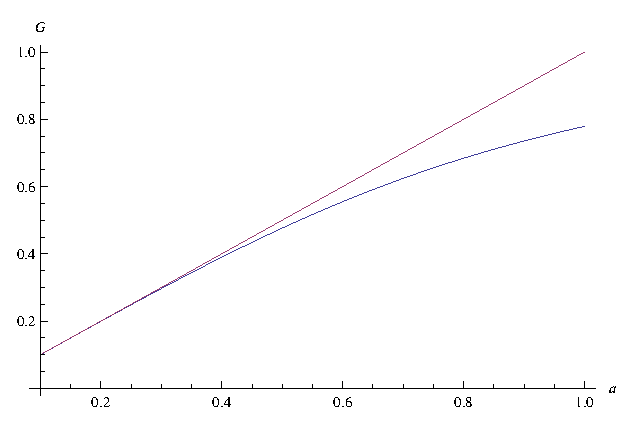
\includegraphics{P_sCDM+LCDM_G.eps}
\caption{Growth factors of sCDM and $\Lambda$CDM}
\end{figure}

\begin{figure}
\centering
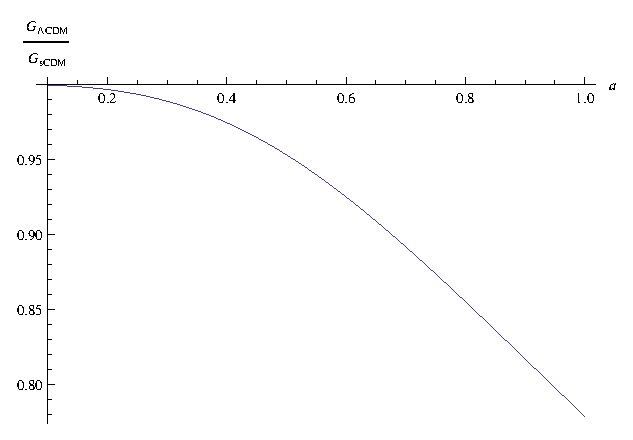
\includegraphics{P_sCDM+LCDM_G2.eps}
\caption{Ratio of the growth factors.($\Lambda$CDM to sCDM.)}
\end{figure}




\subsubsection{DE}

Similar calculations generate the growth factor for dark energy model (figure \ref{DE_G}) and the difference between sCDM and dark energy model(figure \ref{DE+sCDM_G}).{\footnote{{\color{red}
These are calculated using Mathematica. The mathematica notebook file is located in the same folder of the {\LaTeX} file. Brief notations are given in that file.
}}}

\begin{figure}[h]
\centering
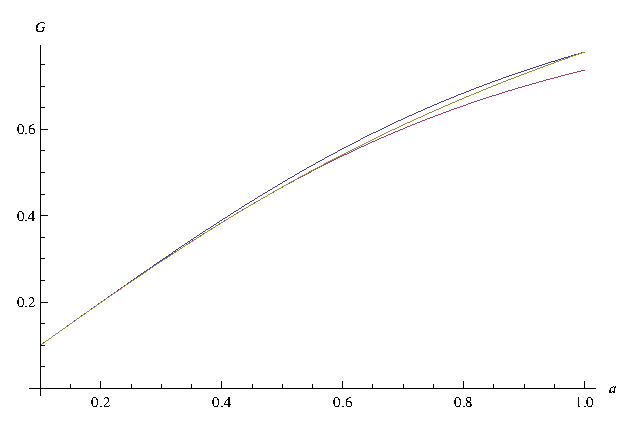
\includegraphics{P_DE_Growth.eps}
\caption{Growth factors of dark energy models with different EoS. The blue line,  red line and green line stand for $w=-0.9$, $w=-1.0$ (it reduces to $\Lambda$CDM model) and $w=-1.1$ respectively.} \label{DE_G}
\end{figure}

\begin{figure}[h]
\centering
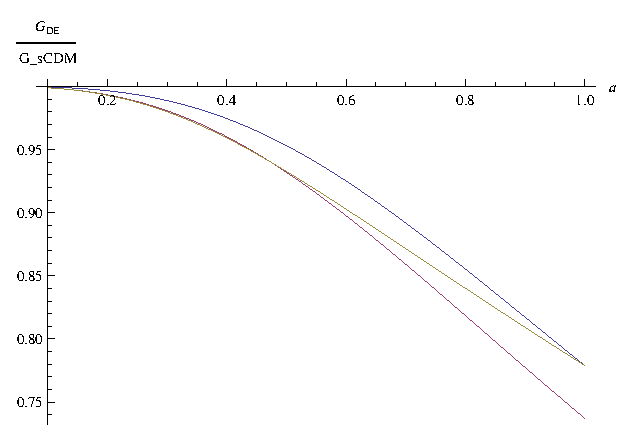
\includegraphics{P_DE+sCDM_G.eps}
\caption{The ratio of growth factors of dark energy model to that of sCDM model.The blue line,  red line and green line stand for $w=-0.9$, $w=-1.0$ (it reduces to $\Lambda$CDM model) and $w=-1.1$ respectively. }\label{DE+sCDM_G}
\end{figure}


\subsubsection{f(R)}
\subsubsection{DGP}
\subsubsection{CPL}
\subsubsection{Interacting?}




\subsection{Power Spectrum}

Calculate the power spectrum of a fiducial model using CMBEASY. {\color{red}I did a little calculation, but it seemed the data never went right. I will check this later.}









\newpage    %It is weird that this command solve the problem that the figure goes between the double line and the text.
\hrule\vspace{1pt}\hrule
\begin{center}
\mbox{{\bf XXXX}} \\
\vspace{0.5em}
\mbox{{XXXX}}
\end{center}
\hrule



\section{Work}

\subsection{Repeat Fernando's work}

\subsubsection{Preparing}

To get the figures in their paper, a figure that describes the relation between growth and the wavenumber $k$ (Growth VS $k$) should be calculated.

\begin{itemize}
\item
Any growth factor can be calculated using the method in previous section.

\item
The next work is to calculate the Hubble distance (because this determines when do the perturbations come into the horizon) of scale factor.

Hubble distance is 
\footnote{
For more details check the {\it Cosmology Projects} notebook}
\begin{equation}
d_H=\int^{a}_{0}{ \frac{\mathrm d a'}{a'^2H(a')} }
\end{equation}

Then we can use the current $d_H(a(t_0))$ and MD approximation of $H(a(t))$ (since we will only cal. the MD evolution of the perturbations.) 
\footnote{
There are many things to be considered. 
\begin{itemize}
\item 
Different models might give different evolution of Hubble distance. And what is knotty is that the models might give different current value of Hubble distance when given a suitable set of parameters (because one might focus on other things to fit the parameters). (???) 

\end{itemize}}

$H(a(t))$ can be simplified into 
\begin{equation}
H(a)=H_0 (\Omega_{M0}a^{-3}+\Omega_{DE0}a^{-3(1+w)})
\end{equation}
according the fact that current observation shows the universe is filled with 73\% dark energy and 27\% matter (mostly dark matter).

\end{itemize}


\subsubsection{$\Lambda$CDM}

Parameters
\begin{eqnarray*}
w=-1;\Omega _{\text{DE0}}=0.734;\Omega _{\text{k0}}=0;\Omega _{\text{m0}}=0.1334\left/\left(0.71^2\right)\right.;\Omega _{\text{r0}}=8.09*10^{-5};
\end{eqnarray*}

Hubble distance:
\begin{figure}[!htbp]
\centering
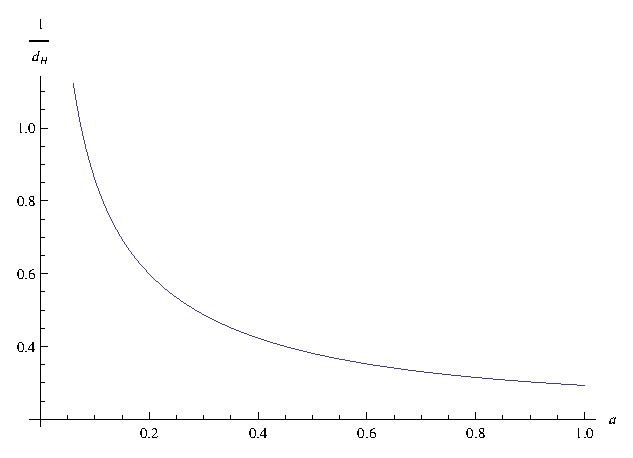
\includegraphics[width=400pt]{P_LCDM_HubbleDistance.eps}
\caption{$\frac{1}{d_H}$ vs $a$}
\end{figure}

growth factor:
\begin{figure}[!htbp]
\centering
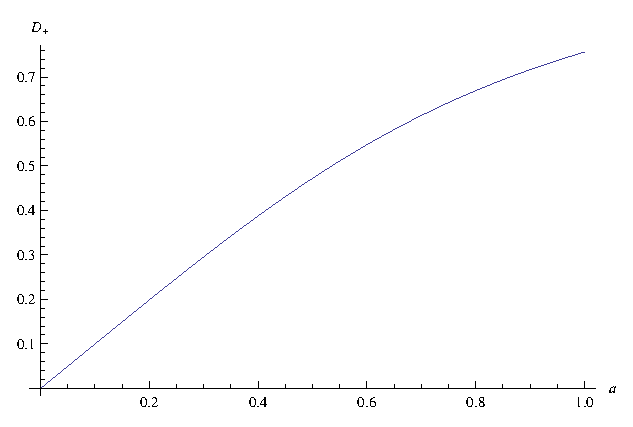
\includegraphics[width=400pt]{P_LCDM_Growth.eps}
\caption{growth factor}
\end{figure}

Growth vs $k$
\begin{figure}[!htbp]
\centering
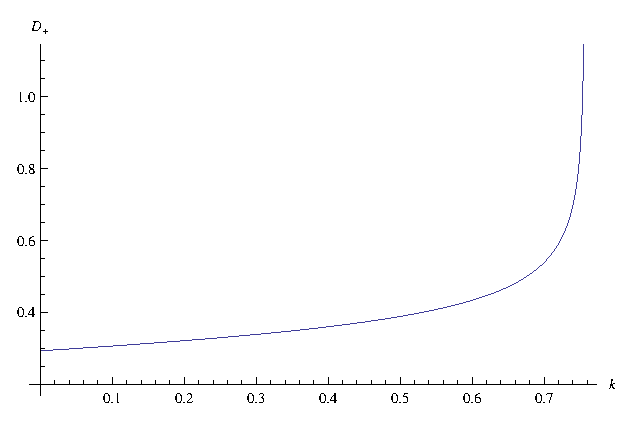
\includegraphics[width=400pt]{P_LCDM_GrowthVSk.eps}
\caption{Growth}
\end{figure}




\subsubsection{LCDM and Dark Energy}

Parameters are listed below.

\begin{eqnarray}
&\Omega _{\text{DE0}}=0.734;\Omega _{\text{k0}}=0;\Omega _{\text{m0}}=0.1334\left/\left(0.71^2\right)\right.;
\Omega _{\text{r0}}=8.09*10^{-5};
\\
&\Omega _{\text{m0},s}=1;\Omega _{\text{r0},s}=8.09*10^{-5};\\
&h=0.71;H_0=\frac{100 h}{300000};
\end{eqnarray}

Each color in the figures represents a model.
\vspace{2ex}
\begin{center}
\begin{tabular}{|c|c|}\hline
{\bf Color} & {\bf Model} \\\hline
Red & sCDM \\\hline
Orange & LCDM \\\hline
Yellow & $w=-0.25$ \\ \hline
Green &  $w=-0.5$ \\ \hline
Blue & $w=-0.75$ \\ \hline
\end{tabular}
\end{center}
\vspace{2ex}





\begin{figure}[!htbp]
\centering
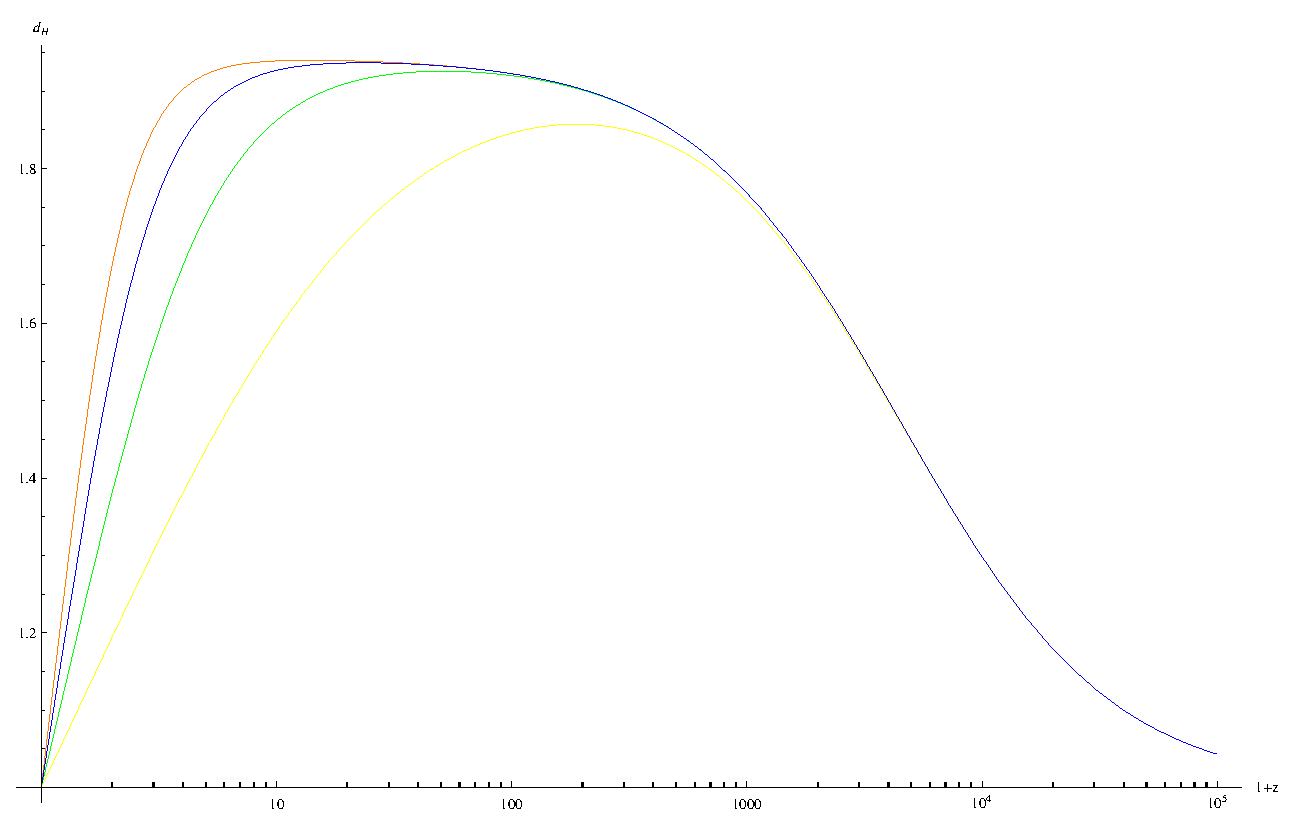
\includegraphics[width=400pt]{DE_HubbleDistances.eps} 
\caption{Hubble distances}\label{fig:DE_HubbleDistances}
\end{figure}


Figure \ref{fig:DE_HubbleDistances} shows the differences of the evolution of the Hubble distance. All the data are normalised with the inverse of sCDM's Hubble distance.
The shape of the lines can be explained by the fact that DE or Lambda only changes the background of the universe at late times after RD. The reason for the dropping down of the lines is that the Hubble functions should have the same value today ($1+z=1$). That is also the reason for the fact that they cross the same point at $1+z=1$. (Values of Hubble equations should converge at late times. So the part with $1+z<1$ is useless.)

Through figure \ref{fig:DE_HubbleDistances} the three DE models fall between LCDM and sCDM which should be a straight line of value 1. Since the EoS of three DE models are exactly between 0 and -1, this result is quite reasonable. This figure also shows that the DE model with $w=-0.25$ obviously deviates from LCDM at an early age of $z\sim 1000$, while other models deviate after about $z\sim 50$.






\begin{figure}[!htbp]
\centering
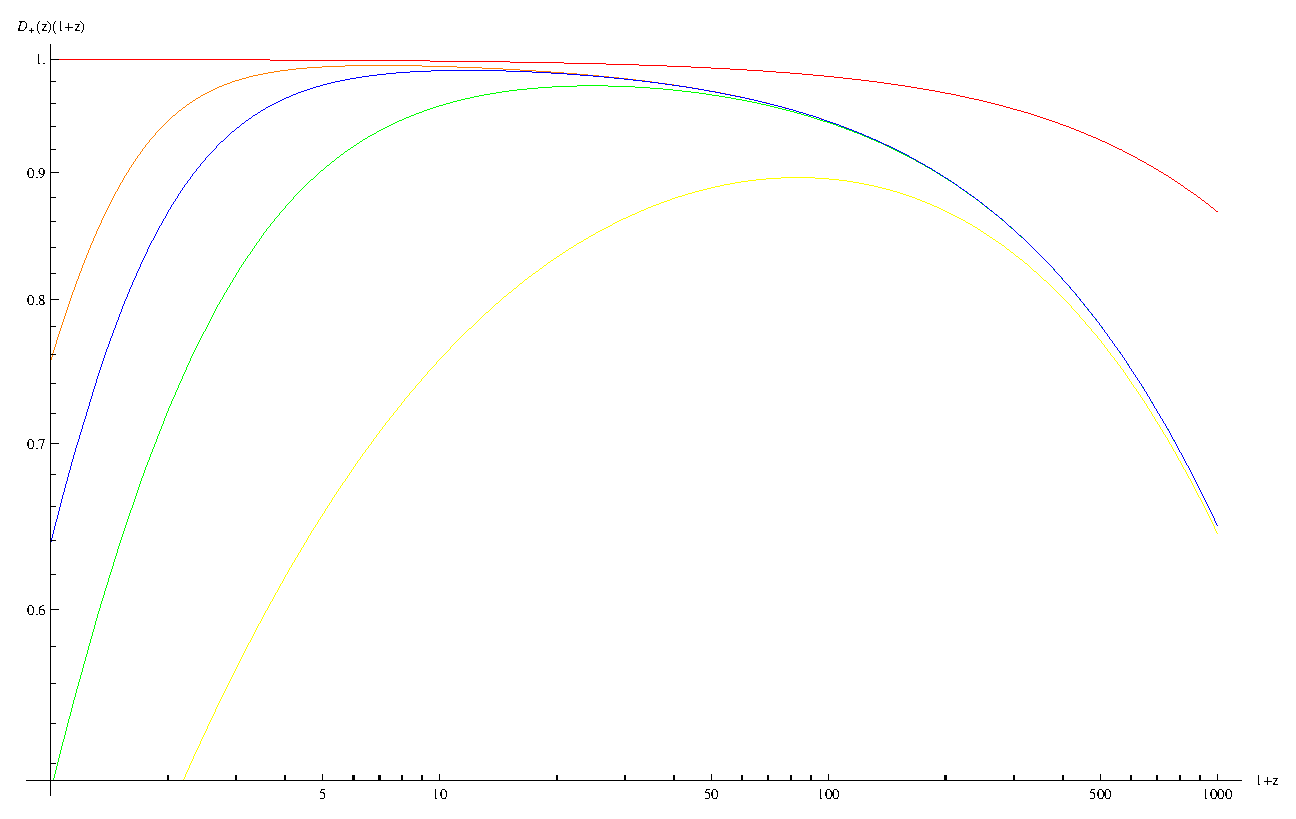
\includegraphics[width=400pt]{DE_GrowthFactors.eps} 
\caption{Growth factors vs $1+z$ of DE and $\Lambda$CDM}\label{fig:DE_GrowthFactors}
\end{figure}


Figure \ref{fig:DE_GrowthFactors} are the growth factors of the models. The going down lines are due to the late age effect of dark energy which suppresses the evolution of perturbations.

[{\color{red}\bf \it Why does the yellow line ($w=-0.25$) behave so strangely? Though we only use the part with $1+z$ larger than 1, it is hard to imagine it crossing LCDM (while other lines crossing nothing).}]






\begin{figure}[!htbp]
\centering
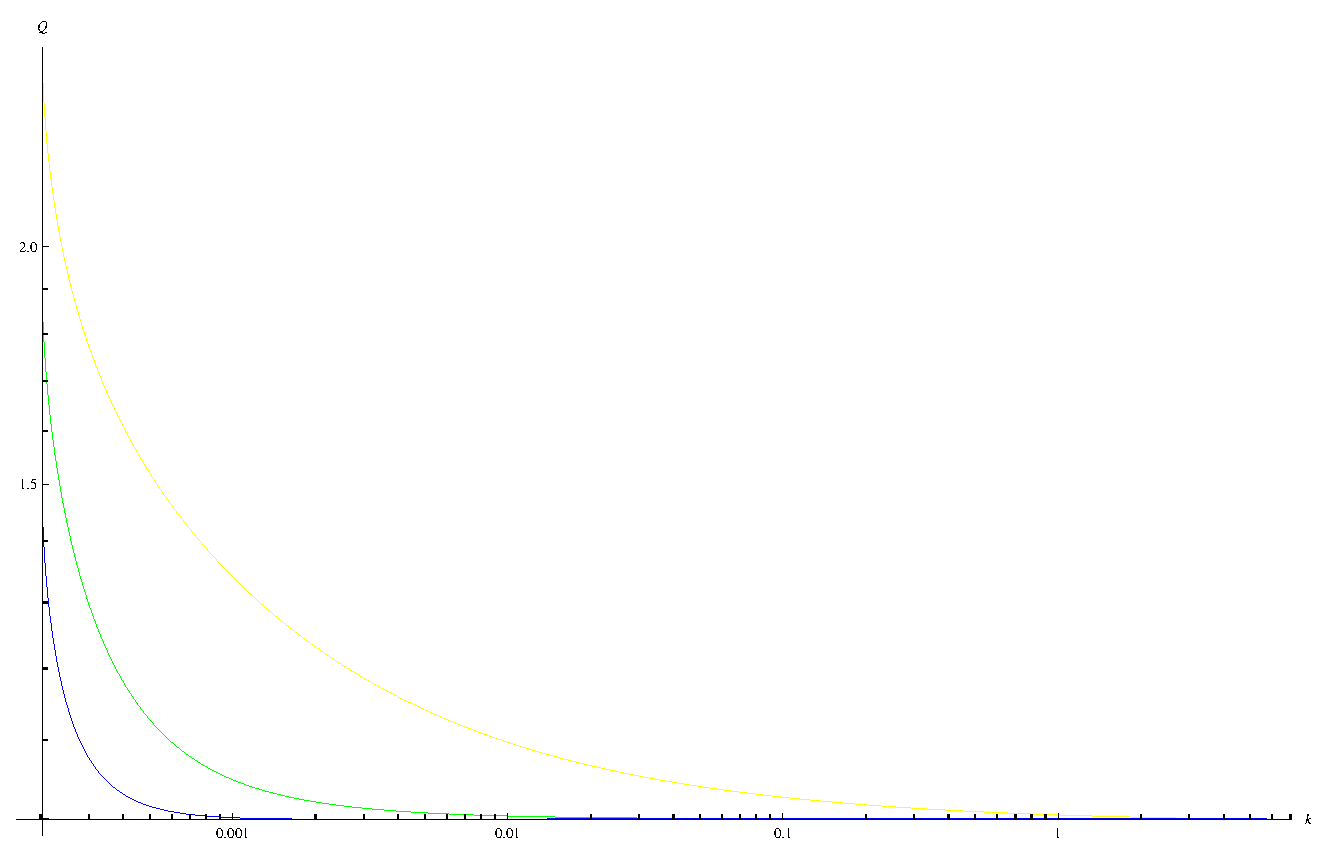
\includegraphics[width=400pt]{DE_QFactors.eps} 
\caption{Q factors}\label{fig:DE_QFactors}
\end{figure}



\begin{figure}[!htbp]
\centering
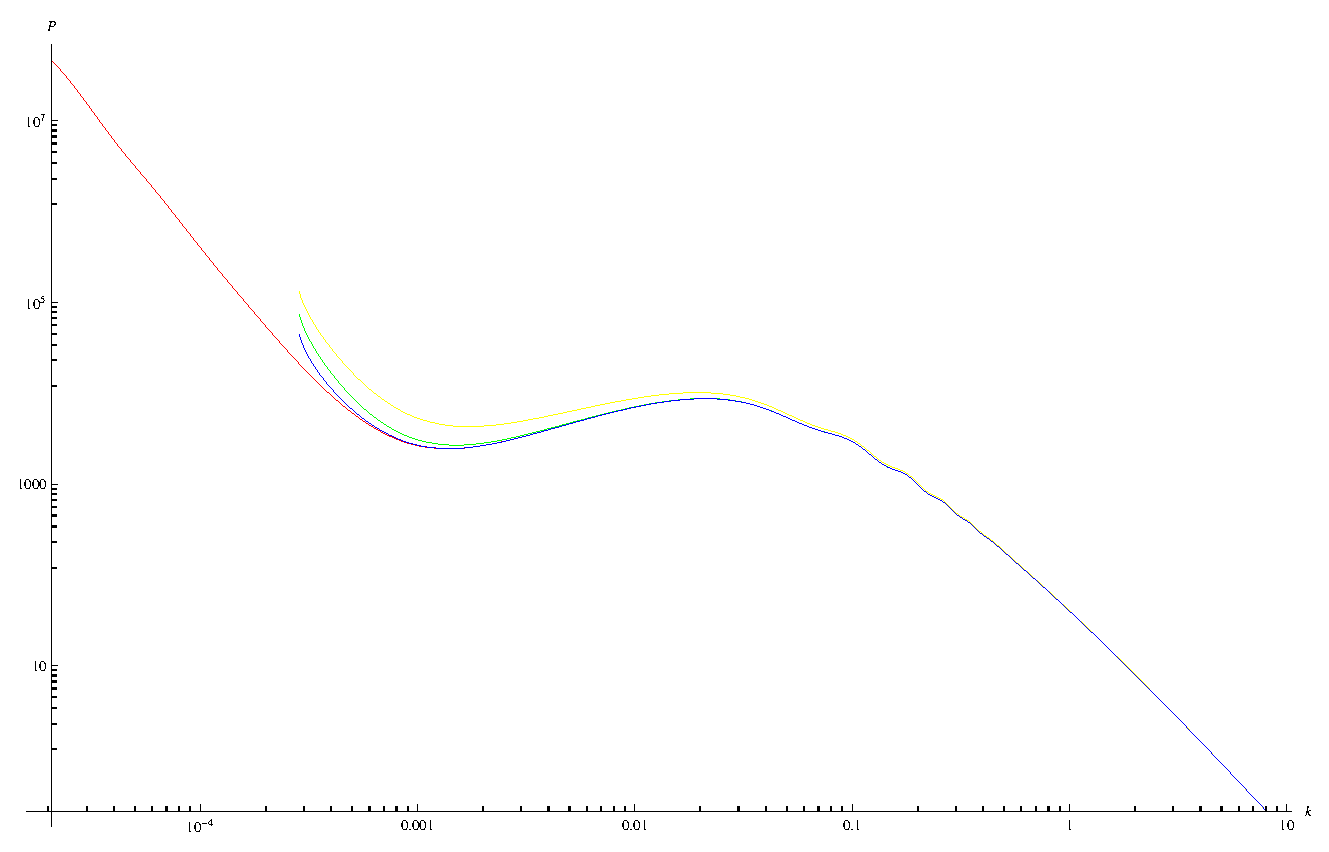
\includegraphics[width=400pt]{DE_PowerSpectrums.eps}
\caption{Power spectrum of LCDM and several DE models}\label{fig:DE_PowerSpectrums}
\end{figure}

\begin{figure}[!htbp]
\centering
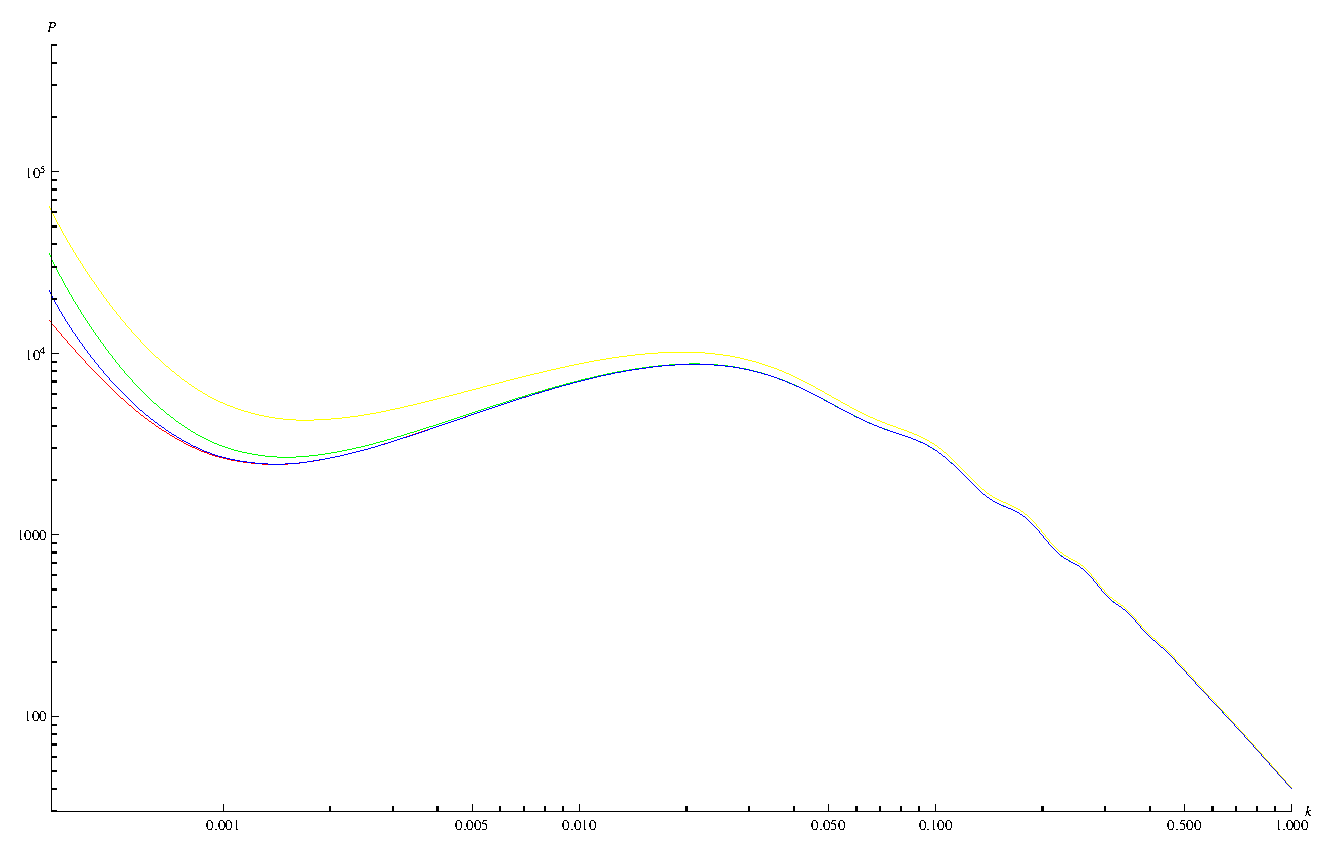
\includegraphics[width=400pt]{DE_PowerSpectrums_Cut.eps}
\caption{Power spectrum (within a range) of LCDM and several DE models}\label{fig:DE_PowerSpectrums_Cut}
\end{figure}



Figure \ref{fig:DE_PowerSpectrums} shows the power spectrums, which are generated by the standard LCDM model. The figure gives the lines the right trend when change the EoS, just as right as the Hubble distance.

One thing that is really annoying is that as the EoS becomes more and more close to LCDM, it is harder and harder to distinguish the DE models with LCDM models. The blue line is a good example for this statement.



These results supports the point that this method works well for these time independent EoS DE models and it can be show the differences of the models in between the time interval we are working on.











\subsection{CPL}


\subsubsection{What Is CPL Parameterisation?}

Notes in {\it Cosmology Project Notebook}.

The EoS here is $w=w_0+w_a(1-a)$.

\subsubsection{Generating Power Sepctrum}

The figures in this subsubsection follows the following rules unless exceptions are stated:
\begin{itemize}
\item
Red for sCDM;orange for LCDM;yellow for 

\end{itemize}

Parameters table (other parameters are exactly the same with the previous calculation):

\vspace{2ex}
\begin{center}
\begin{tabular}{|c|c|}\hline
{\bf Color} & {\bf Model} \\\hline
Red & sCDM \\\hline
Orange & LCDM \\\hline
Yellow & $w_a=-0.20$ \\ \hline
Green &  $w_a=-0.30$ \\ \hline
Blue & $w_a=-0.32$ \\ \hline
Cyan & $w_a=-0.34$ \\ \hline
Purple & $w_a=-0.44$ \\ \hline
\end{tabular}
\end{center}
\vspace{2ex}

In these CPL models, the parameters make sure that $w_0+w_a=-1$ in order to generate a background analogous to LCDM.

It should be made clear that the range of validity is around $10^{-4}<k<10$ or equivalently a range of $10^{-3}<a<1$.




\begin{figure}[!htbp]
\centering
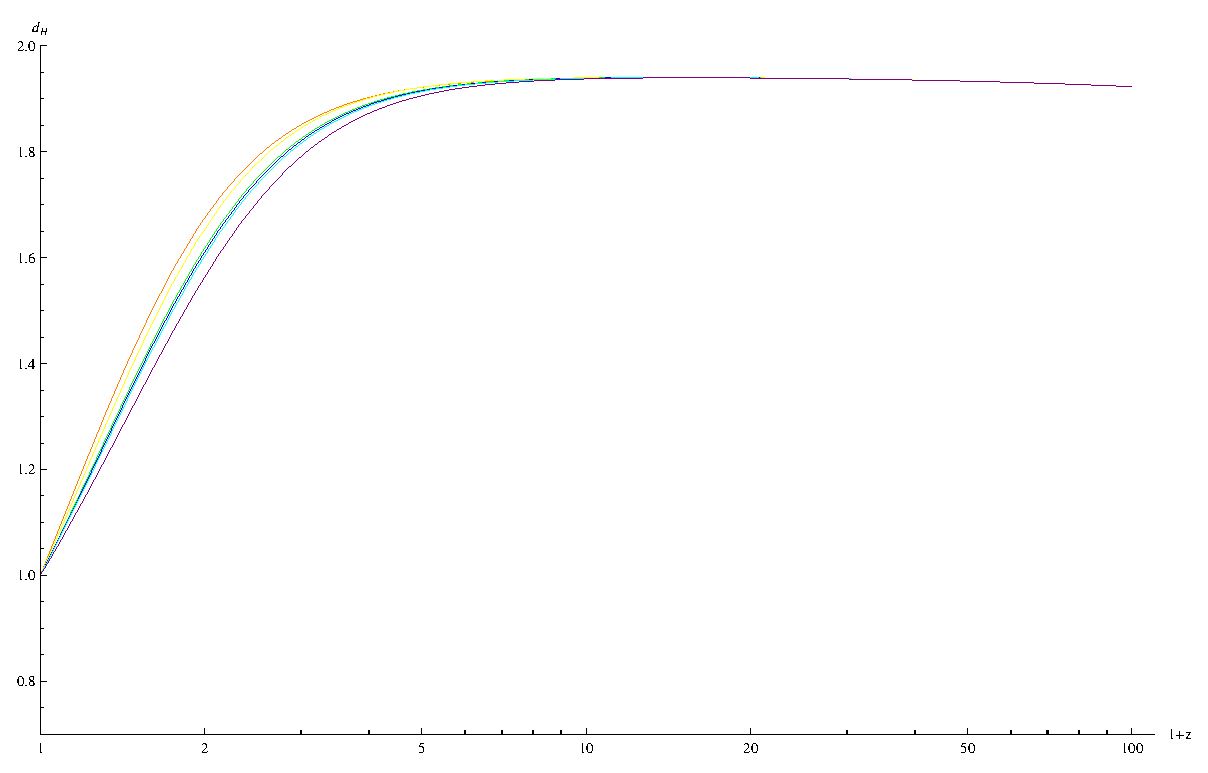
\includegraphics[width=400pt]{CPL_HubbleDistances.eps}
\caption{The Hubble distance of different models including sCDM, LCDM and five other CPL parameterised dark energy model}\label{fig:CPL_HubbleDistances}
\end{figure}

Figure \ref{fig:CPL_HubbleDistances}  shows the Hubble distances. The $1+z<1$ part is also useless so I cut them off. The smaller the EoS is, the larger the Hubble distance is during late ages. The parameters chosen here are all fits to LCDM well. So the difference between between them is small. However the differences are large enough to be noticed.



\begin{figure}[!htbp]
\centering
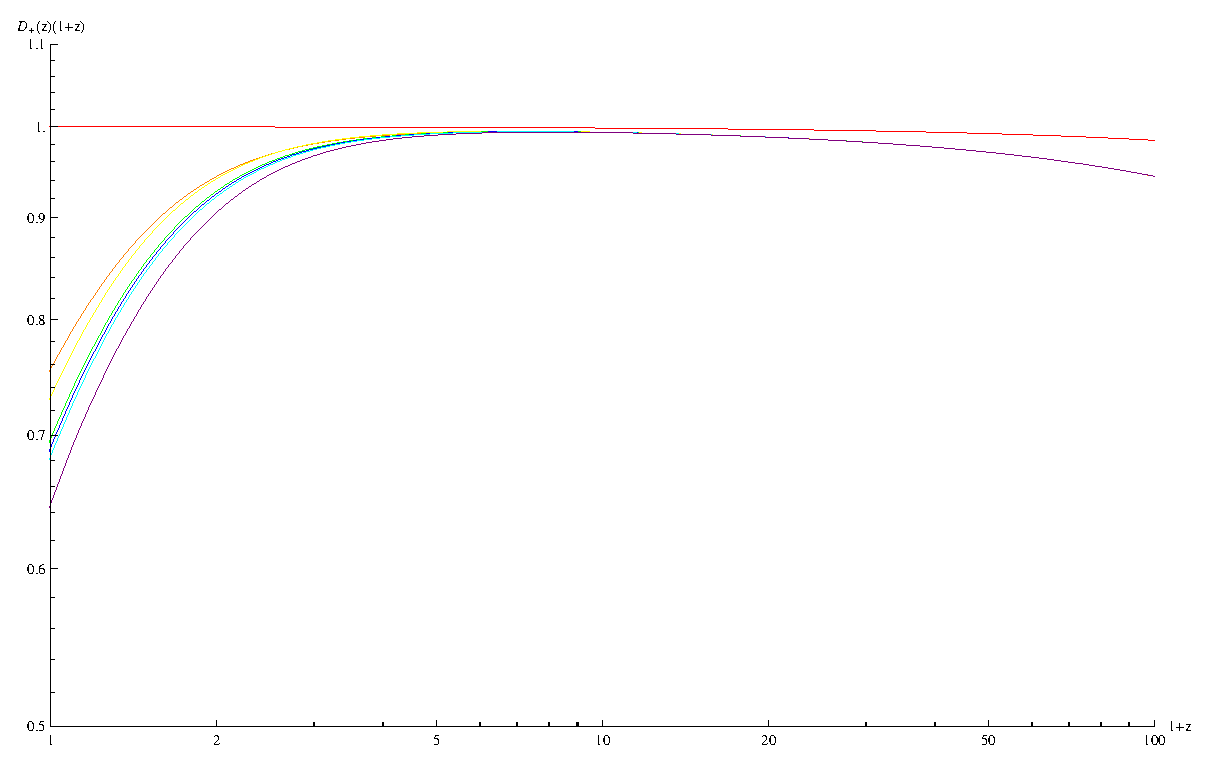
\includegraphics[width=400pt]{CPL_GrowthFactors.eps}
\caption{The growth factors of different models including sCDM, LCDM and five other CPL parameterised dark energy model}\label{fig:CPL_GrowthFactors}
\end{figure}



\begin{figure}[!htbp]
\centering
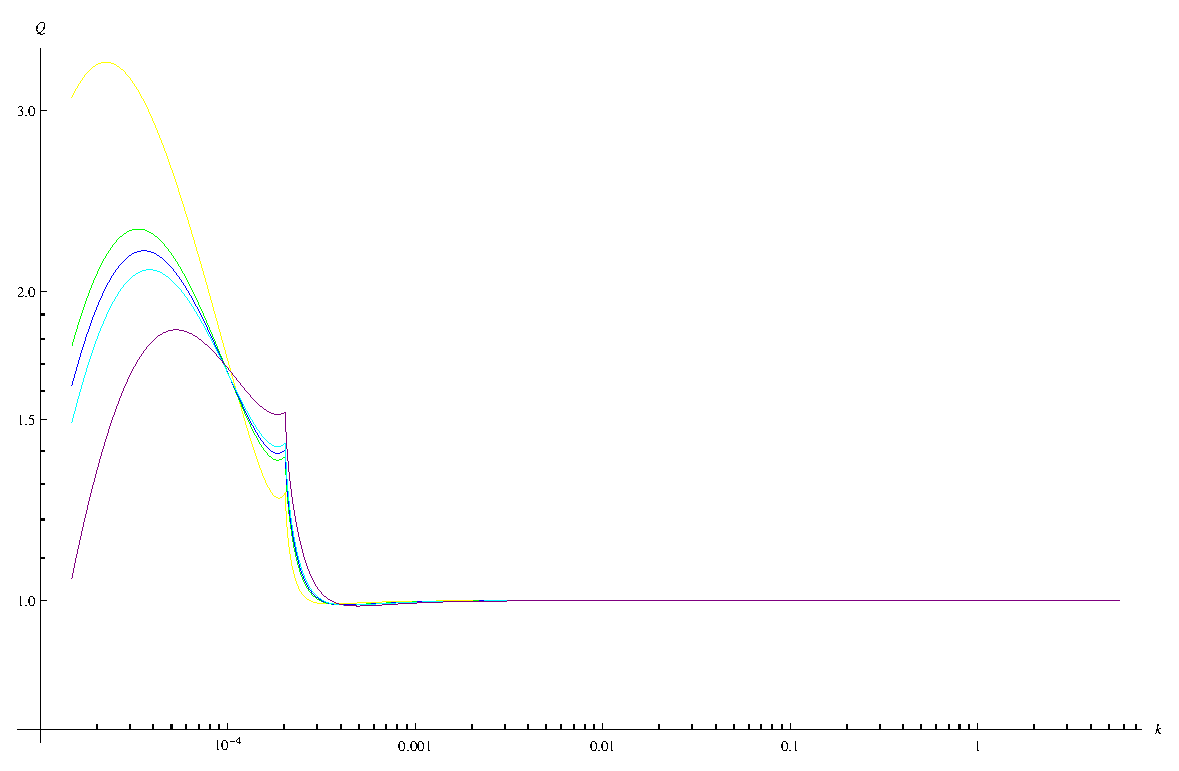
\includegraphics[width=400pt]{CPL_QFactors.eps}
\caption{The Q factors of different models including sCDM, LCDM and five other CPL parameterised dark energy model}\label{fig:CPL_QFactors}
\end{figure}





\begin{figure}[!htbp]
\centering
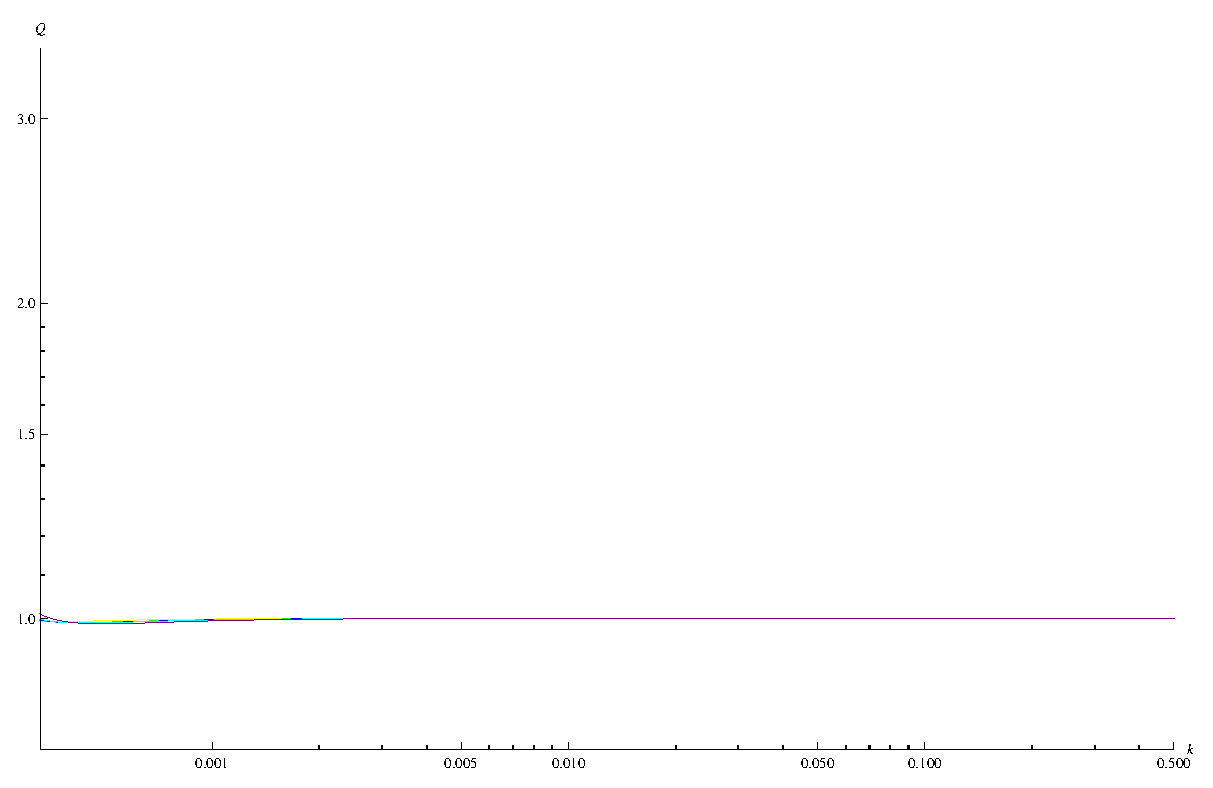
\includegraphics[width=400pt]{CPL_QFactors_Cut.eps}
\caption{The Q factors (within a range) of different models including sCDM, LCDM and five other CPL parameterised dark energy model}\label{fig:CPL_QFactors_Cut}
\end{figure}

Figure \ref{fig:CPL_GrowthFactors} has peaks. These peaks comes from the $1+z<1$ part of the growth factor. These should be cut off latter.

The figures show the smaller the parameters $w_a$, the larger deviation from LCDM at late times.




\begin{figure}[!htbp]
\centering
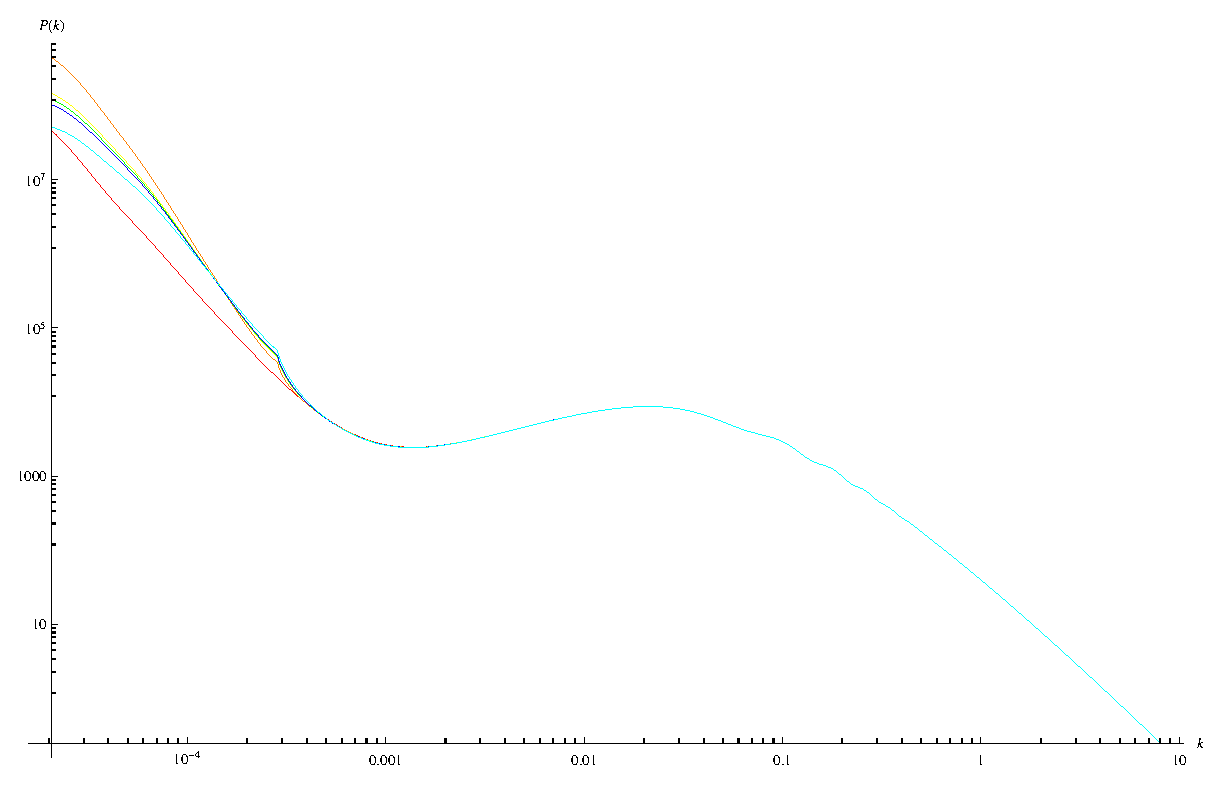
\includegraphics[width=400pt]{CPL_PowerSpectrums.eps}
\caption{The power spectrums of different models including sCDM, LCDM and five other CPL parameterised dark energy model}\label{fig:CPL_PowerSpectrums}
\end{figure}





\begin{figure}[!htbp]
\centering
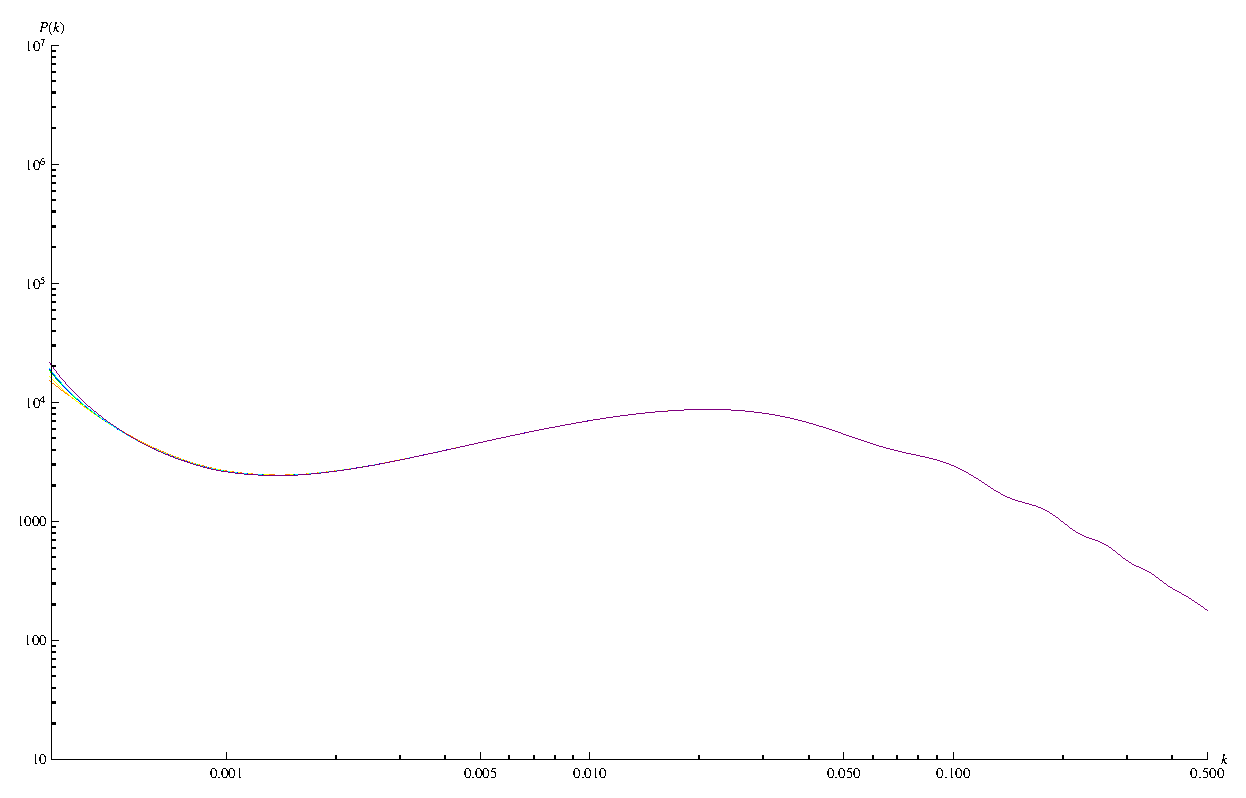
\includegraphics[width=400pt]{CPL_PowerSpectrums_Cut.eps}
\caption{The power spectrums (within a range) of different models including sCDM, LCDM and five other CPL parameterised dark energy model}\label{fig:CPL_PowerSpectrums_Cut}
\end{figure}





Figure \ref{fig:CPL_PowerSpectrums_Cut} shows that the power spectrum can hardly be recognised until today. (I am making too small changes in the parameters. More references needed here in order make this clear.)








\subsection{\color{blue}First Supplements}


\begin{quotation}
{\color{blue}


\begin{enumerate}

\item\label{item:HubbleDistance}

\begin{figure}[!htpb]
\centering
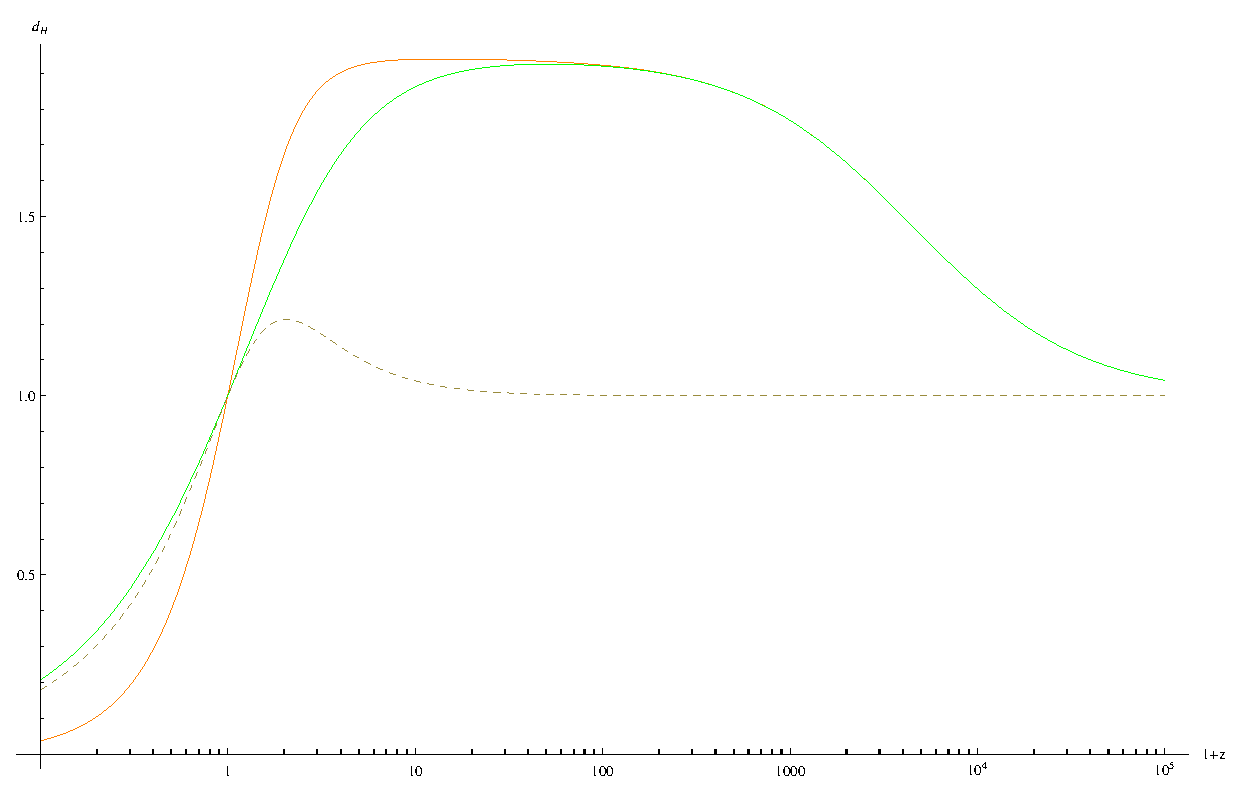
\includegraphics[width=350pt]{DE_Supp_HubbleDistances.eps}
\caption{\color{blue}Hubble distance. Dashed line is the Hubble distance ratio of DE (with $w=-0.5$) and LCMD.}\label{fig:DE_Supp_HubbleDistances}
\end{figure}

Figure \ref{fig:DE_Supp_HubbleDistances} corresponds to Figure 1 {a} in Fernando's. I think $1+z<1$ is of nonsense because redshift $z$ should be larger than 1 if we only care about the present and the past. So I only plotted the $1+z>1$. Here my figure is different from Fernando's at about $1+z<10$. All the lines converge at $z=0$ in my plot because all the Hubble functions becomes the Hubble constant of today at that redshift. I have no idea why Fernando's plot do not. (And I have no idea why he plotted $z<0$).


\item
As said in the previous item, redshift less than zero is not so usefull.

\item
I have already check the effect of $\Omega_{m0}$ and $\Omega_{de0}$. The figure does not change very much.

\begin{figure}[!htpb]
\centering
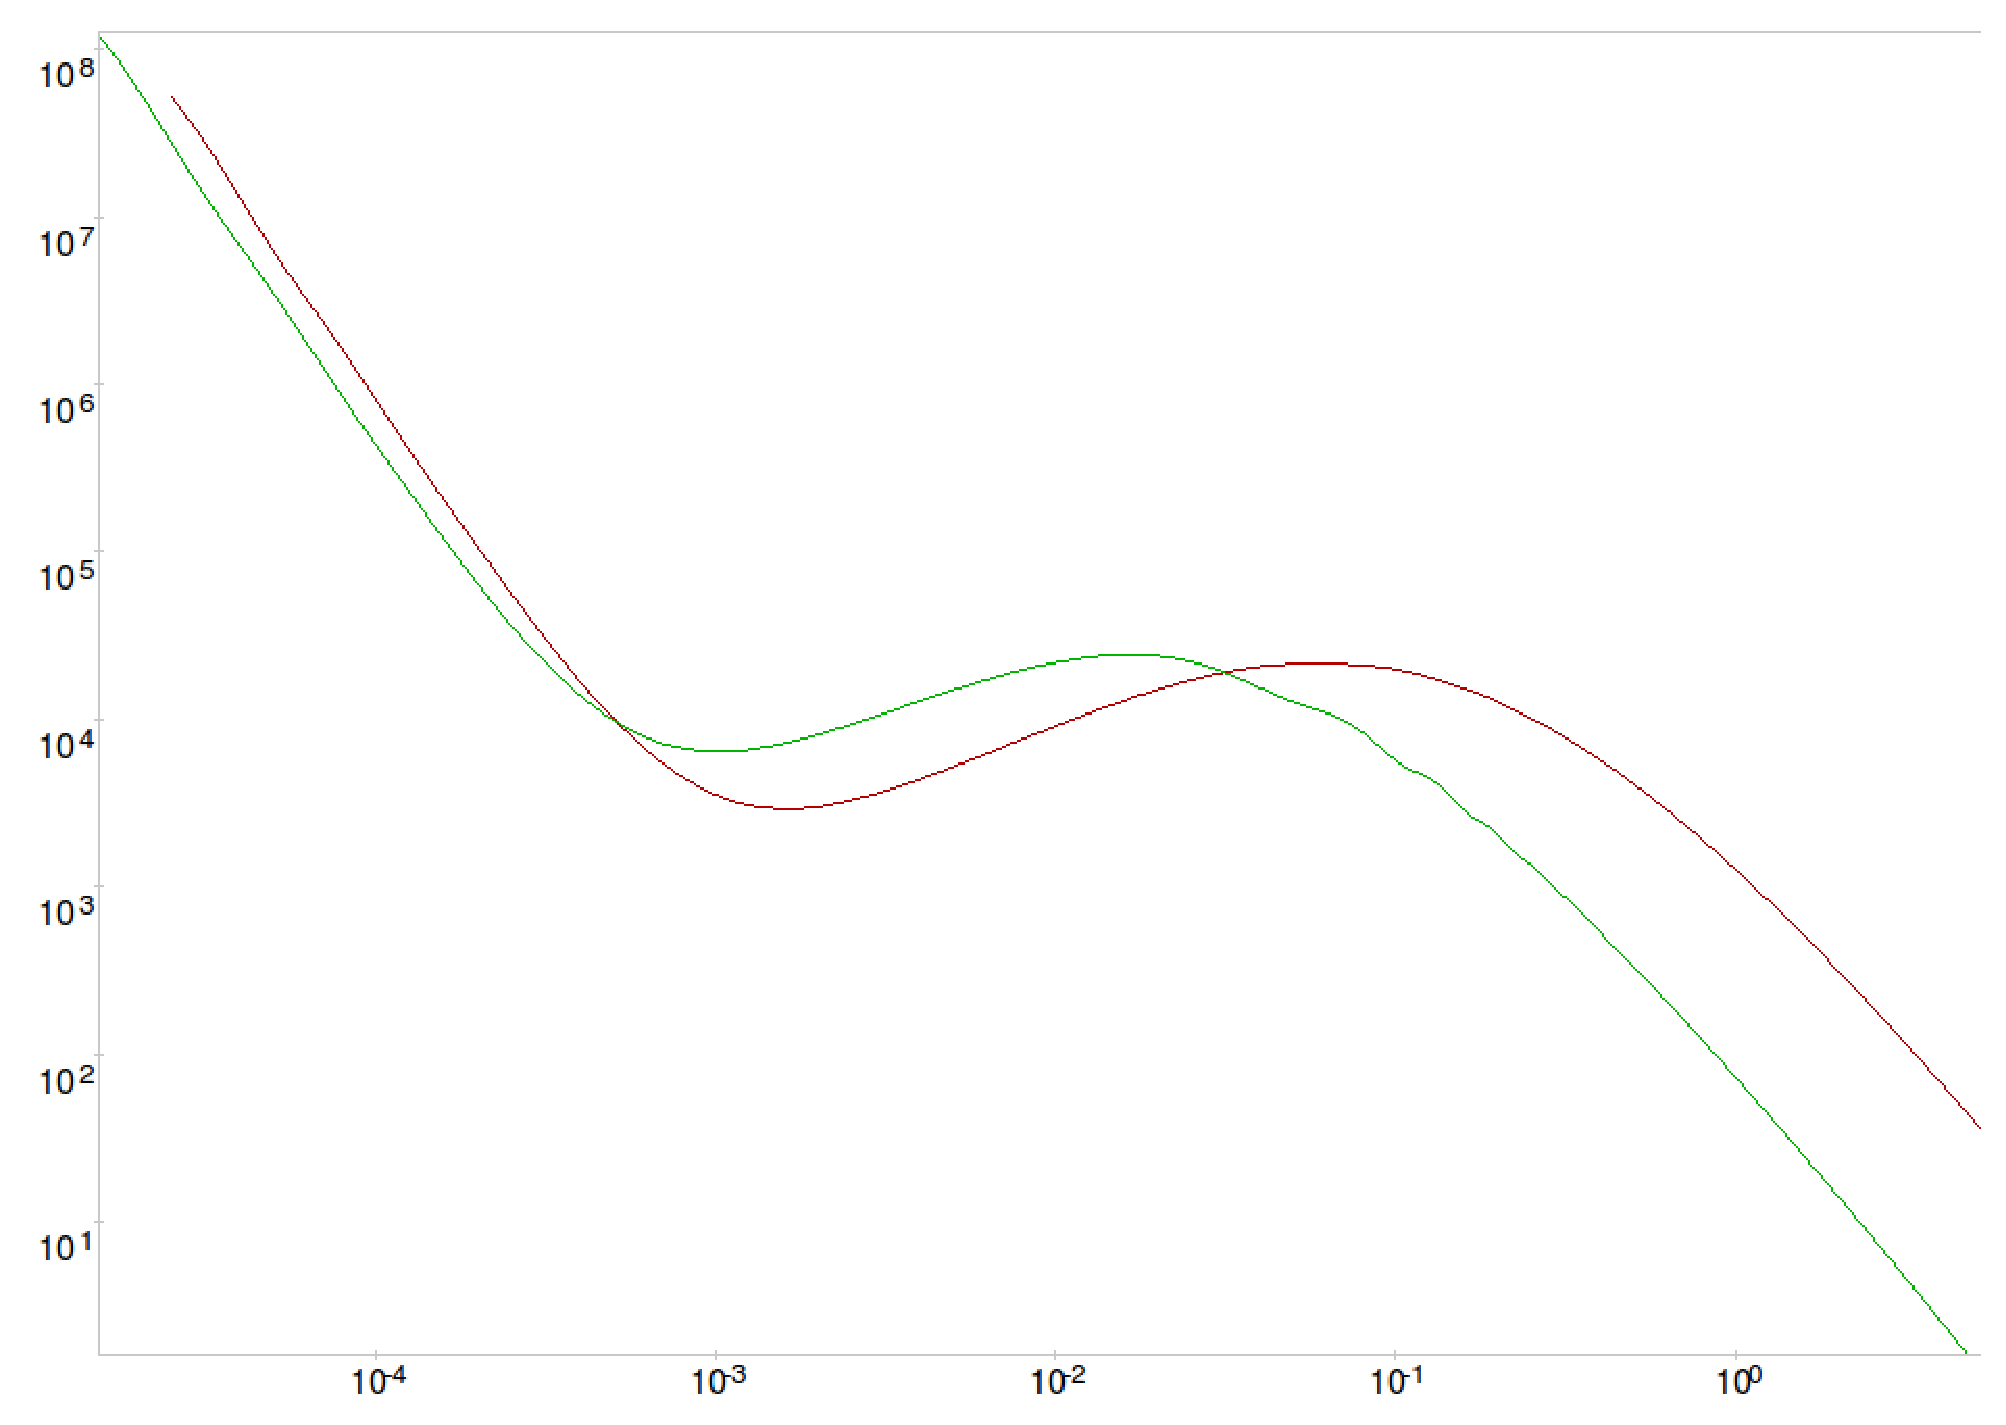
\includegraphics[width=350pt]{PowerSpectrumDEsCDMCMBEASY.eps}
\caption{\color{blue}Power spectrum of dark energy model with $\Omega_{DE0}=0$ and $\Omega_{DE0}=0.7$. The red line is the sCDM model.}
\end{figure}

That's why I did not plot figure varying in $\Omega_{DE0}$.

\item
I think there is no need to plot figures on different DE and DM abundances. Is there anything to be expected from plotting these figures?

Small $k$ corresponds to negative redshift.

\item


\begin{figure}[!htpb]
\centering
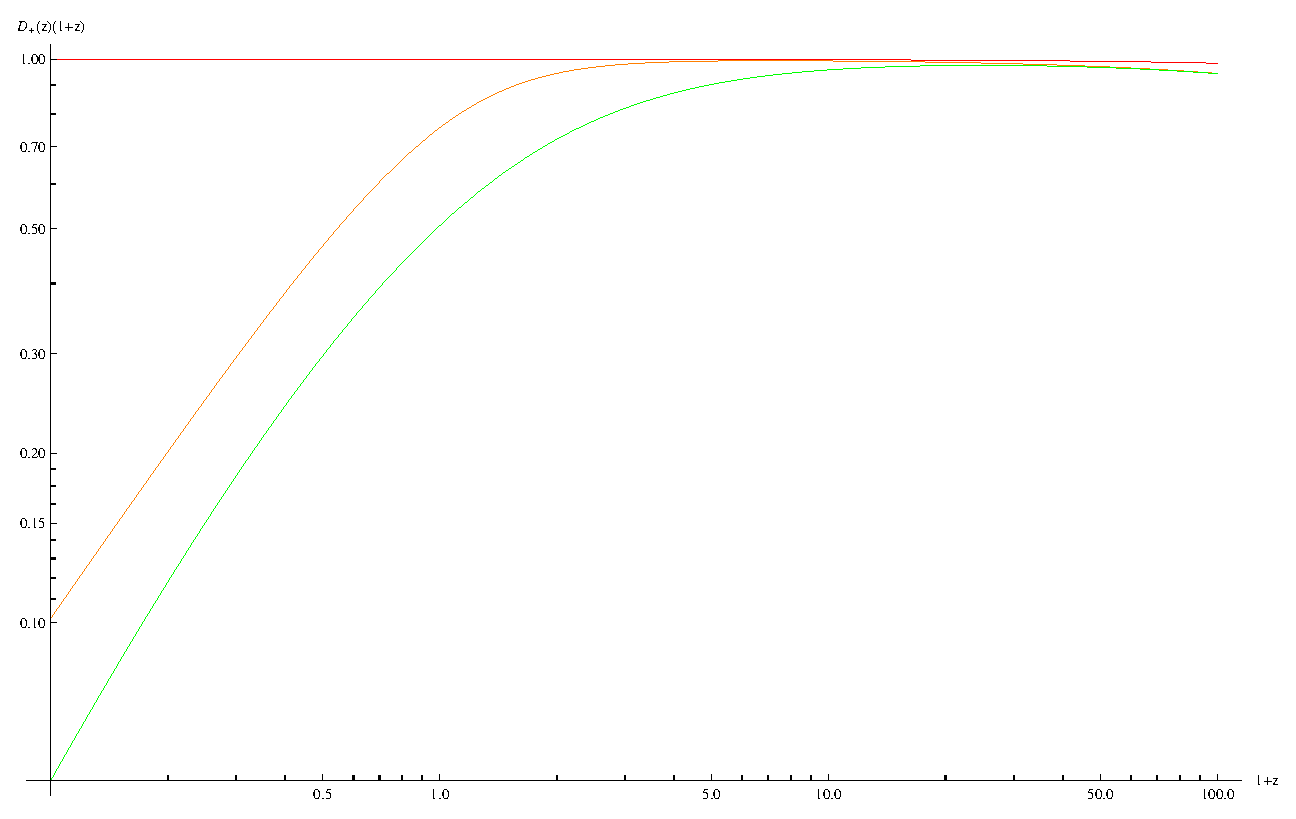
\includegraphics[width=350pt]{DE_Supp_GrowthFactors.eps}
\caption{\color{blue}Growth factors are given in this figure. Dashed line is the Hubble distance ratio of DE (with $w=-0.5$) and LCMD.}\label{fig:DE_Supp_GrowthFactors}
\end{figure}

The growth factors in figure \ref{fig:DE_Supp_GrowthFactors} is plotted within $1+z\sim[0.1,1000]$. As argued in \ref{item:HubbleDistance}, the data is useless when $z<0$ unless one is going to check the future evolution of the universe.
{\bf That is why I give two figures for one quantity sometimes: one for a larger range and one for a suitable range.}



\item

The CPL EoS used here is $w=w_0+w_a(1-a)$. The paramters chosen are listed in the table below.

\vspace{2ex}
\begin{center}
\begin{tabular}{|c|c|}\hline
{\bf Color} & {\bf Model} \\\hline
Red & sCDM \\\hline
Orange & LCDM \\\hline
Yellow & $w_0=-1$ \& $w_a=0.1$ \\ \hline
Green &  $w_0=-1$ \& $w_a=-0.1$ \\ \hline
Blue & $w_0=-0.9$ \& $w_a=-0.1$ \\ \hline
Cyan & $w_0=-0.9$ \& $w_a=0.1$ \\ \hline
Purple & $w_0=-0.9$ \& $w_a=-0.2$ \\ \hline
\end{tabular}
\end{center}
\vspace{2ex}


\begin{figure}[!htpb]
\centering
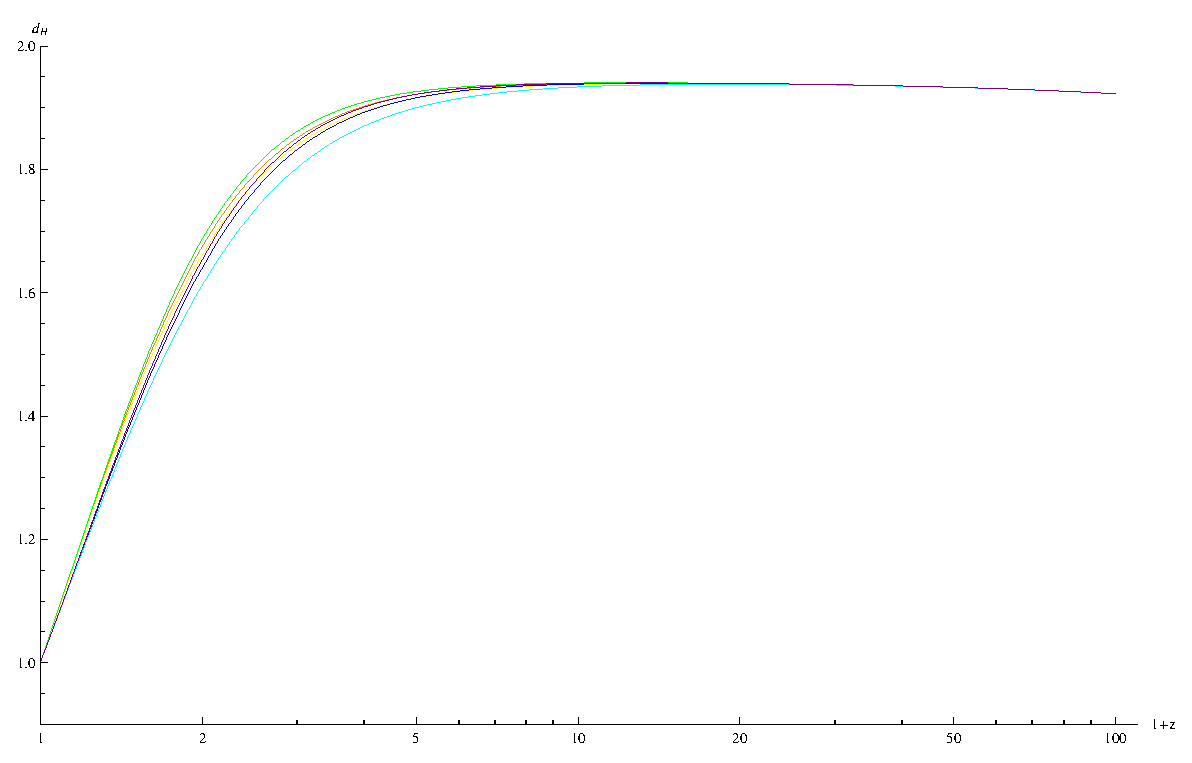
\includegraphics[width=350pt]{CPL_Supp_HubbleDistances.eps}
\caption{\color{blue}Hubble distance of CPL dark energy.}\label{fig:CPL_Supp_HubbleDistances}
\end{figure}

\begin{figure}[!htpb]
\centering
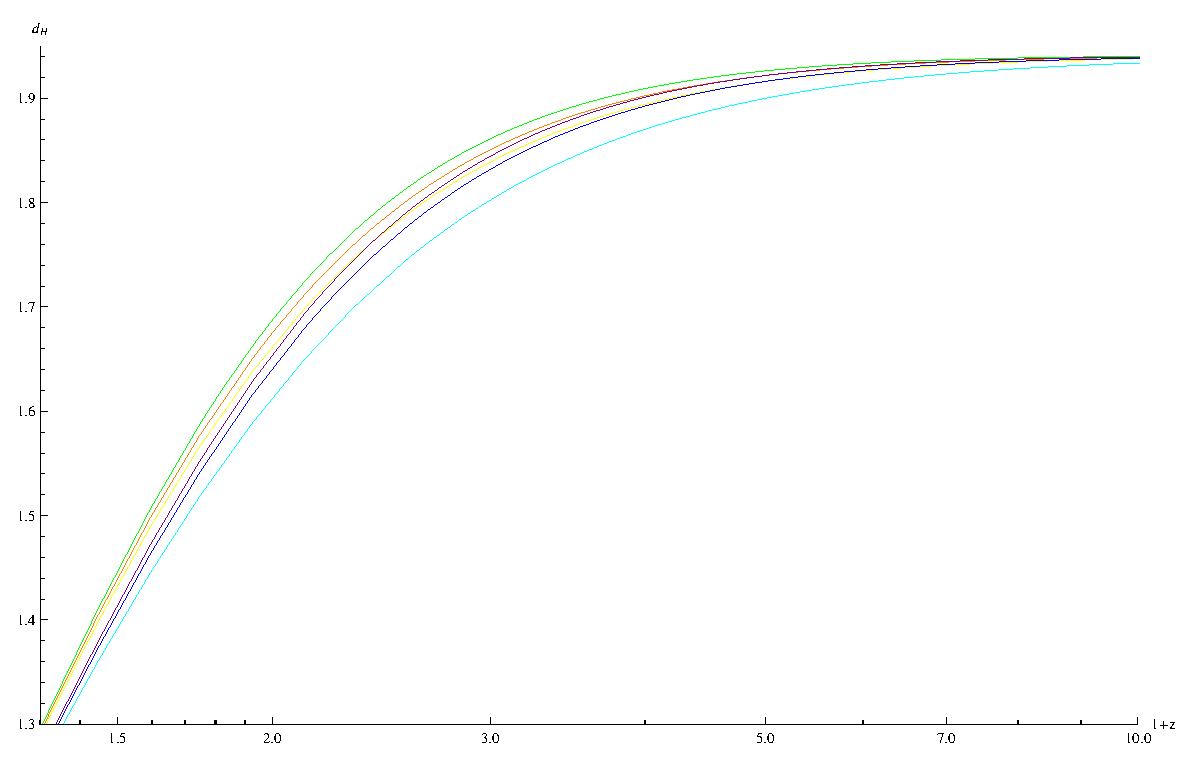
\includegraphics[width=350pt]{CPL_Supp_HubbleDistances_Cut.eps}
\caption{\color{blue}Hubble distance of CPL dark energy.}\label{fig:CPL_Supp_HubbleDistances_Cut}
\end{figure}

\begin{figure}[!htpb]
\centering
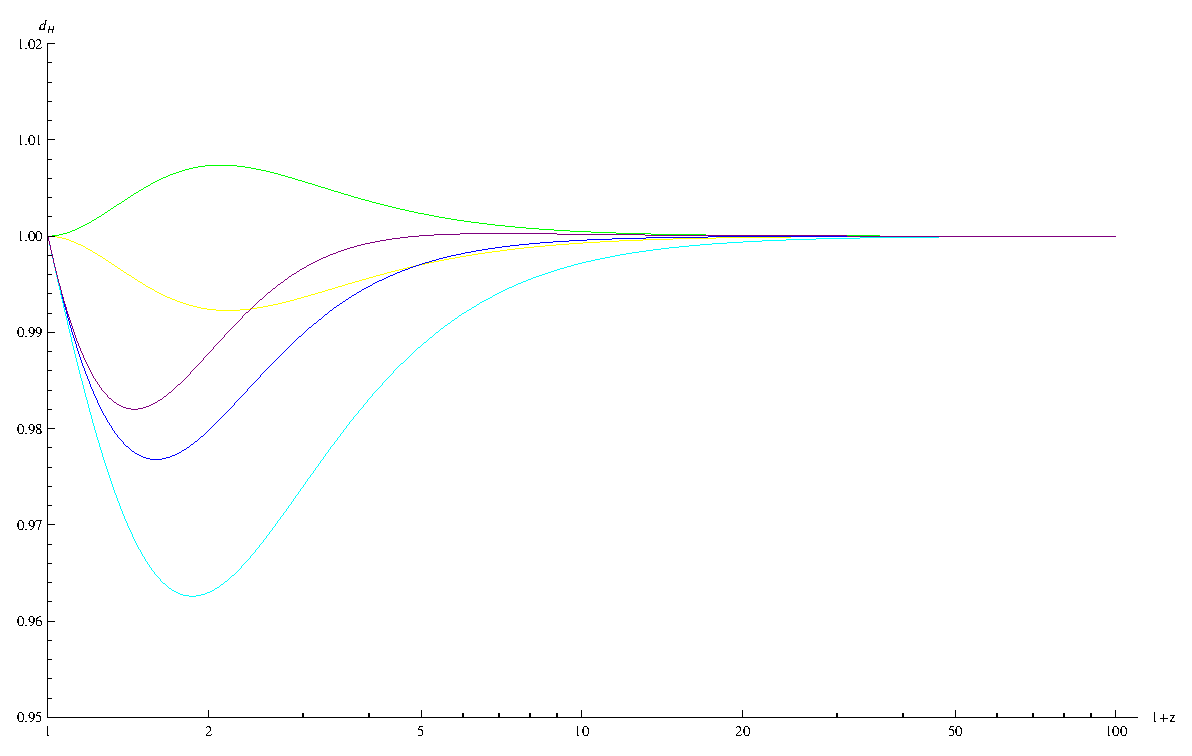
\includegraphics[width=350pt]{CPL_Supp_HubbleDistances_DivideLCDM.eps}
\caption{\color{blue}Hubble distance of CPL dark energy in units of LCDM Hubble distances at the corresponding value.}\label{fig:CPL_Supp_HubbleDistances_DivideLCDM}
\end{figure}

\begin{figure}[!htpb]
\centering
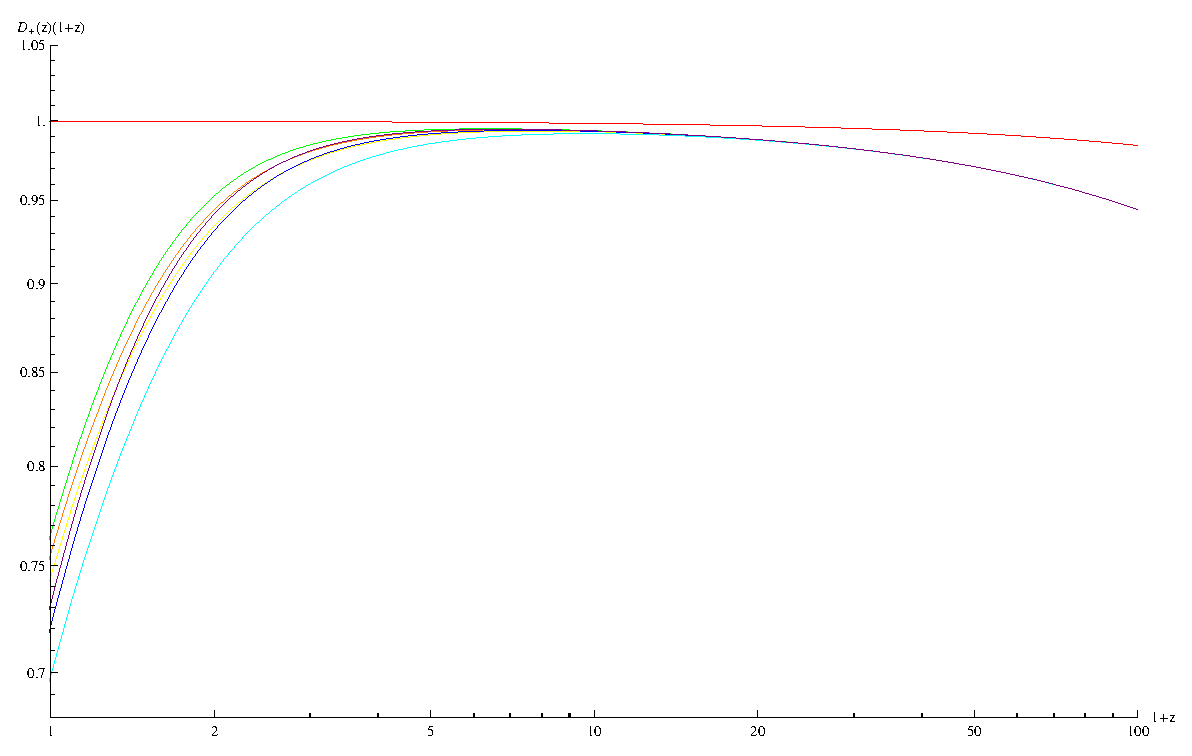
\includegraphics[width=350pt]{CPL_Supp_GrowthFactors.eps}
\caption{\color{blue}Growth factors of CPL dark energy and LCDM in units of sCDM.}\label{fig:CPL_Supp_GrowthFactors}
\end{figure}

\begin{figure}[!htpb]
\centering
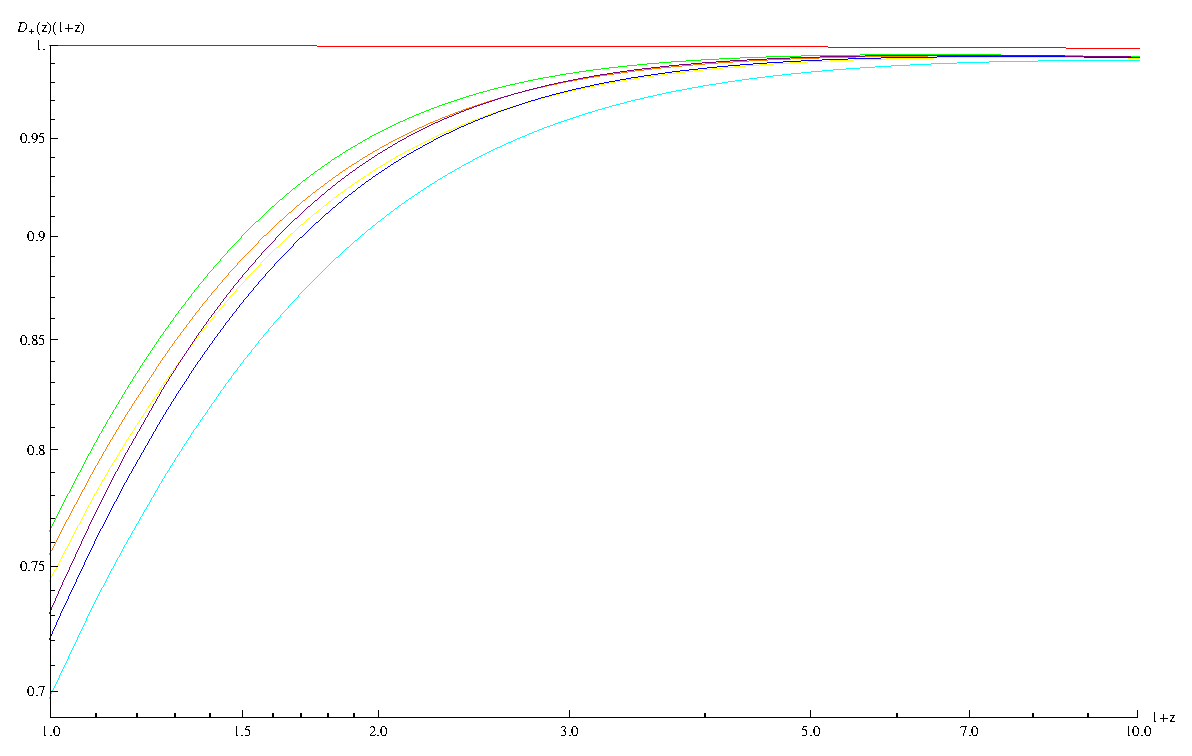
\includegraphics[width=350pt]{CPL_Supp_GrowthFactors_Cut.eps}
\caption{\color{blue}Growth factors of CPL dark energy and LCDM in units of sCDM.}\label{fig:CPL_Supp_GrowthFactors_Cut}
\end{figure}




\begin{figure}[!htpb]
\centering
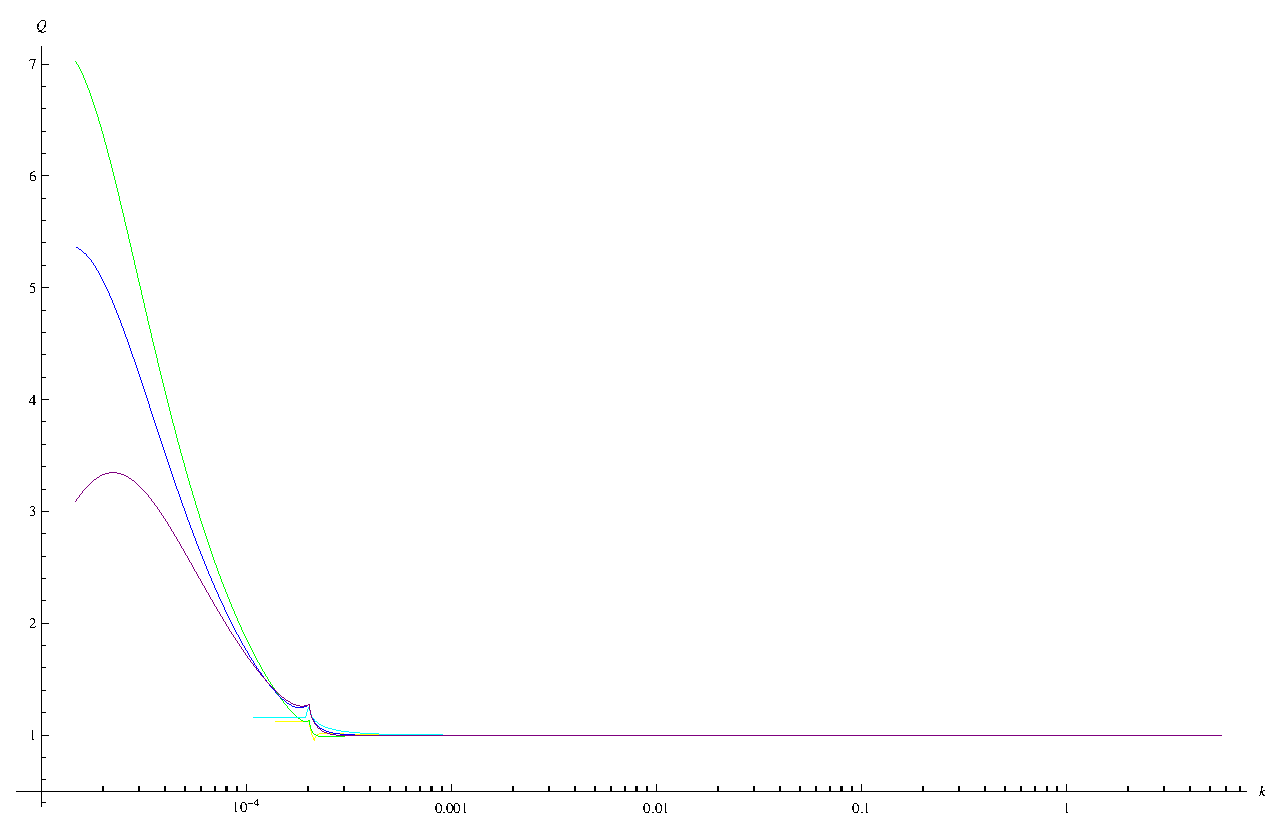
\includegraphics[width=350pt]{CPL_Supp_QFactors.eps}
\caption{\color{blue}Q factors of CPL dark energy and LCDM in units of sCDM.}\label{fig:CPL_Supp_QFactors}
\end{figure}


\begin{figure}[!htpb]
\centering
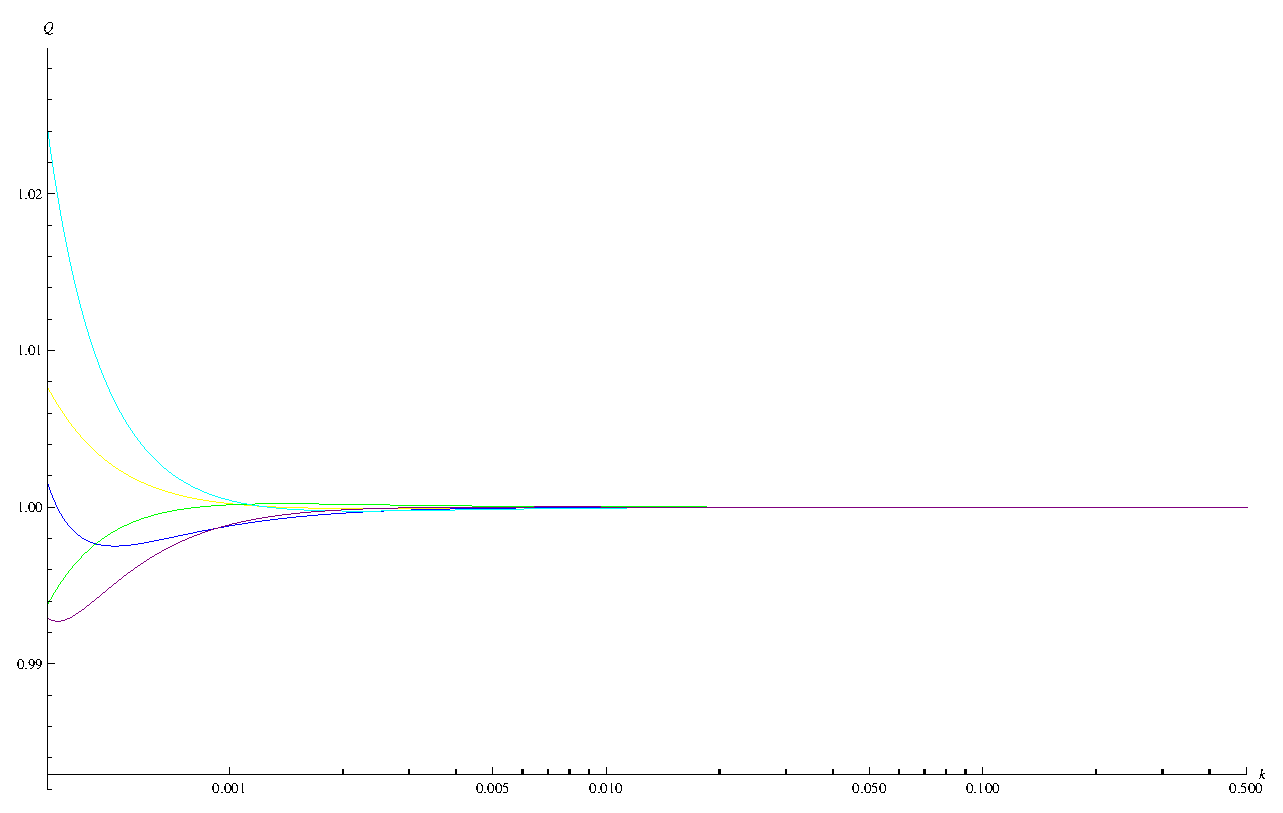
\includegraphics[width=350pt]{CPL_Supp_QFactors_Cut.eps}
\caption{\color{blue}Q factors of CPL dark energy and LCDM in units of sCDM.}\label{fig:CPL_Supp_QFactors_Cut}
\end{figure}

\begin{figure}[!htpb]
\centering
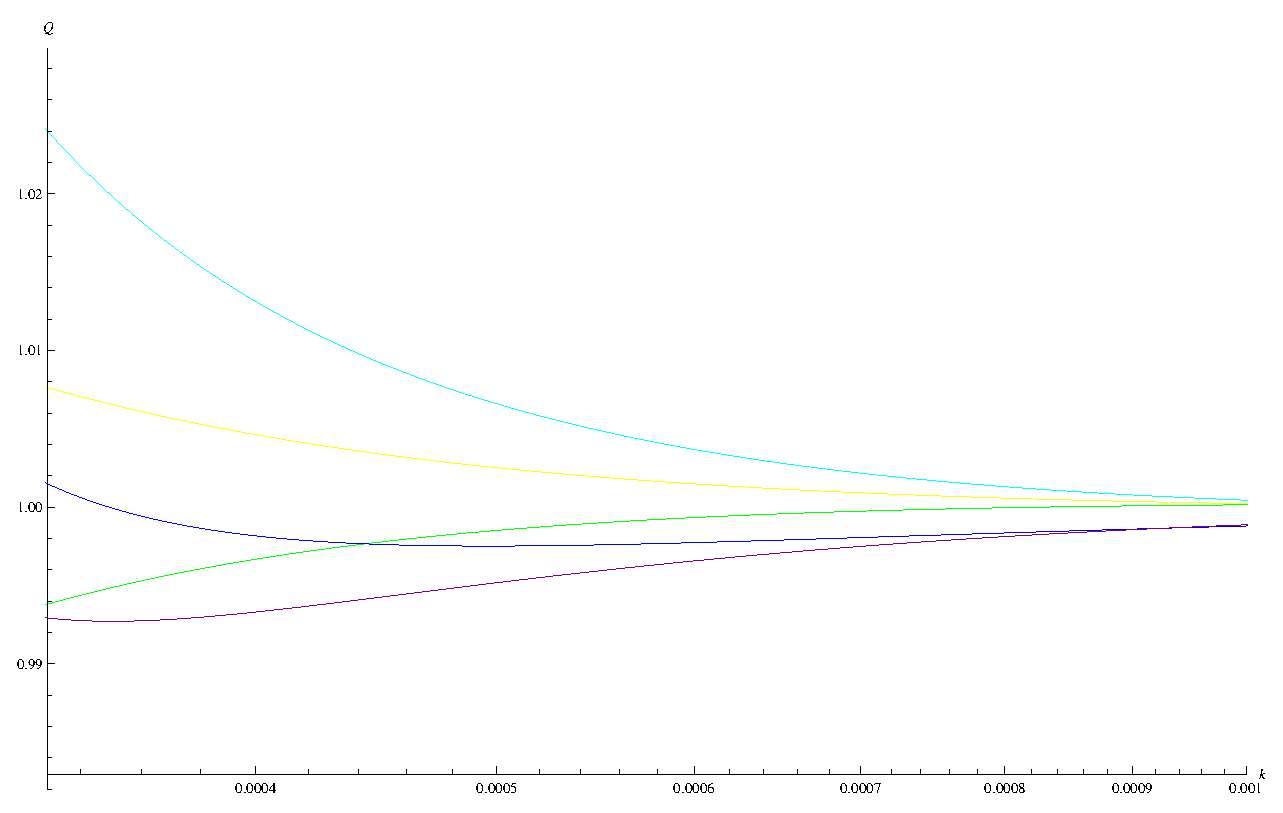
\includegraphics[width=350pt]{CPL_Supp_QFactors_Detail.eps}
\caption{\color{blue}Q factors of CPL dark energy and LCDM in units of sCDM.}\label{fig:CPL_Supp_QFactors_Detail}
\end{figure}


\begin{figure}[!htpb]
\centering
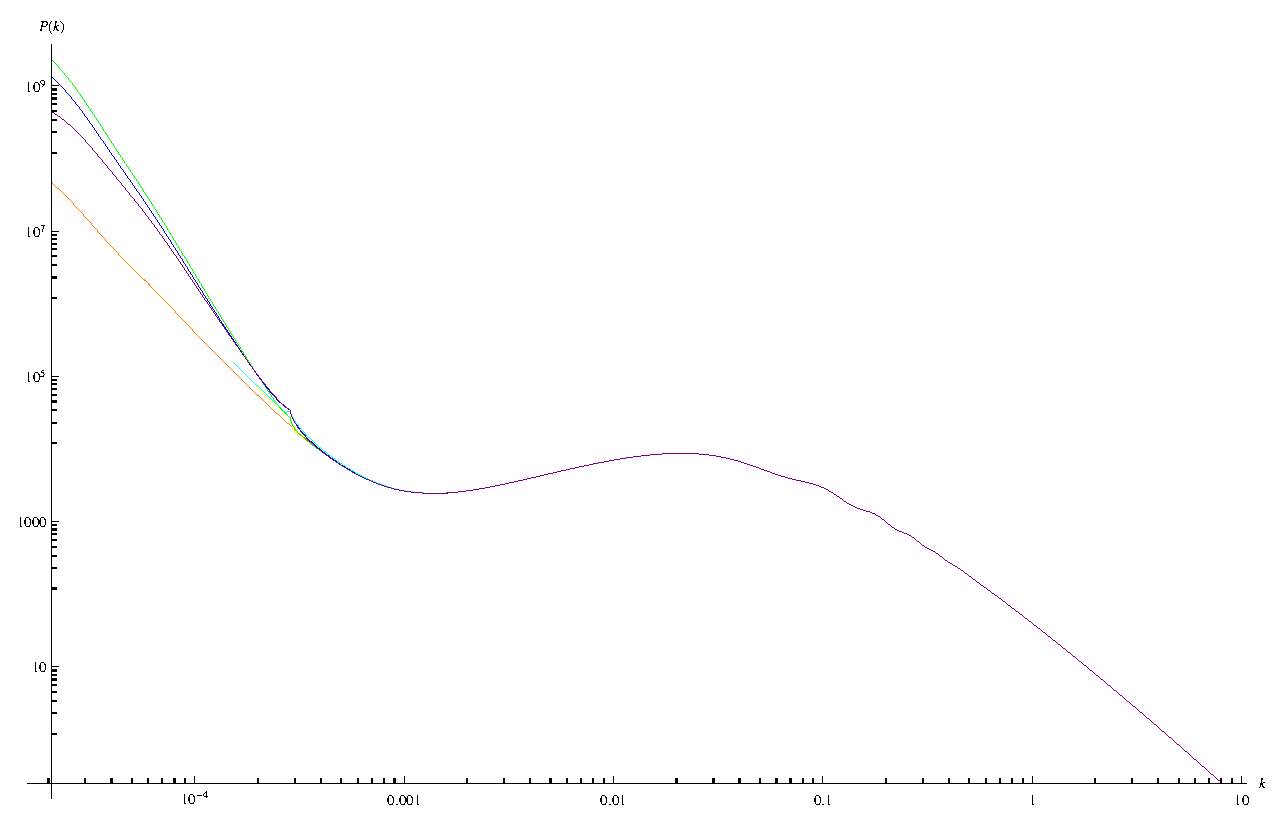
\includegraphics[width=350pt]{CPL_Supp_PowerSpectrums.eps}
\caption{\color{blue}Power spectrum of CPL dark energy and LCDM in units of sCDM.}\label{fig:CPL_Supp_PowerSpectrums}
\end{figure}


\begin{figure}[!htpb]
\centering
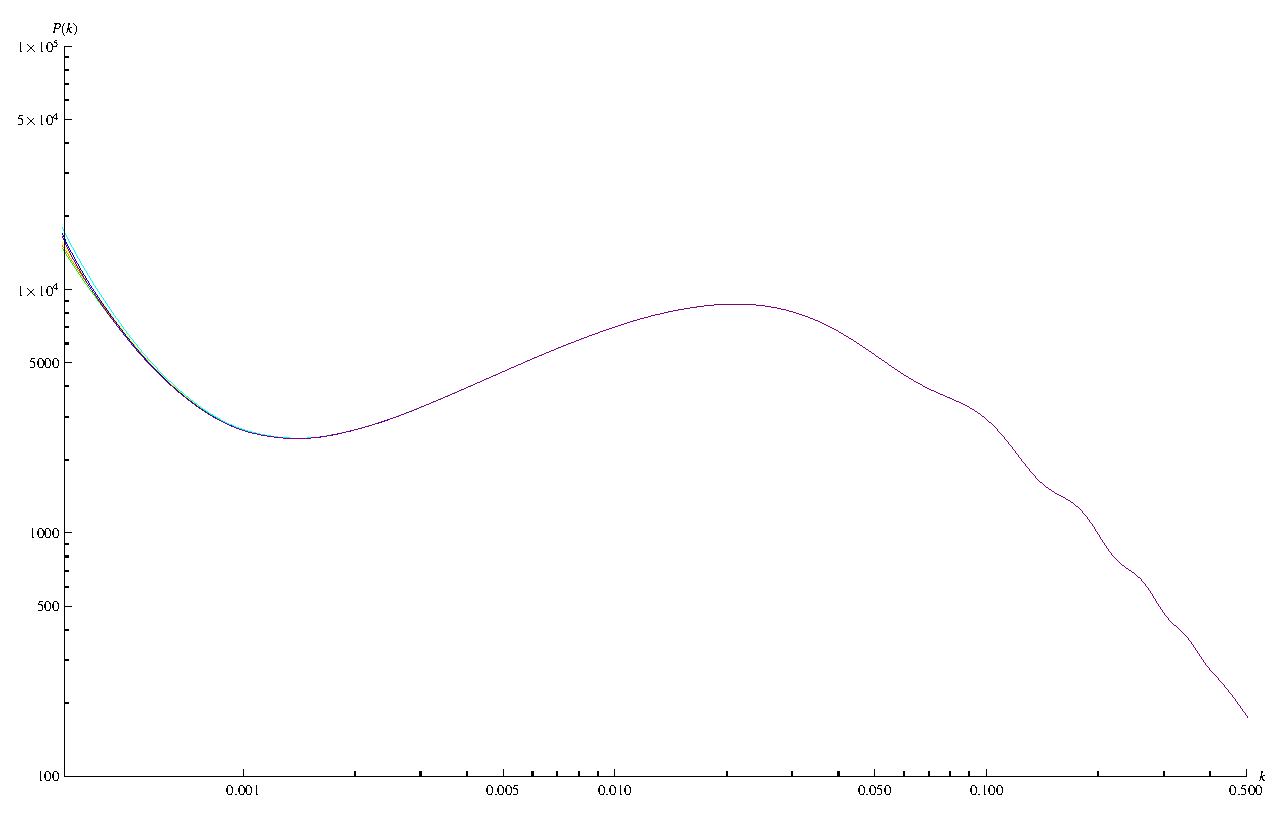
\includegraphics[width=350pt]{CPL_Supp_PowerSpectrums_Cut.eps}
\caption{\color{blue}Power spectrum of CPL dark energy and LCDM in units of sCDM.}\label{fig:CPL_Supp_PowerSpectrums_Cut}
\end{figure}


\begin{figure}[!htpb]
\centering
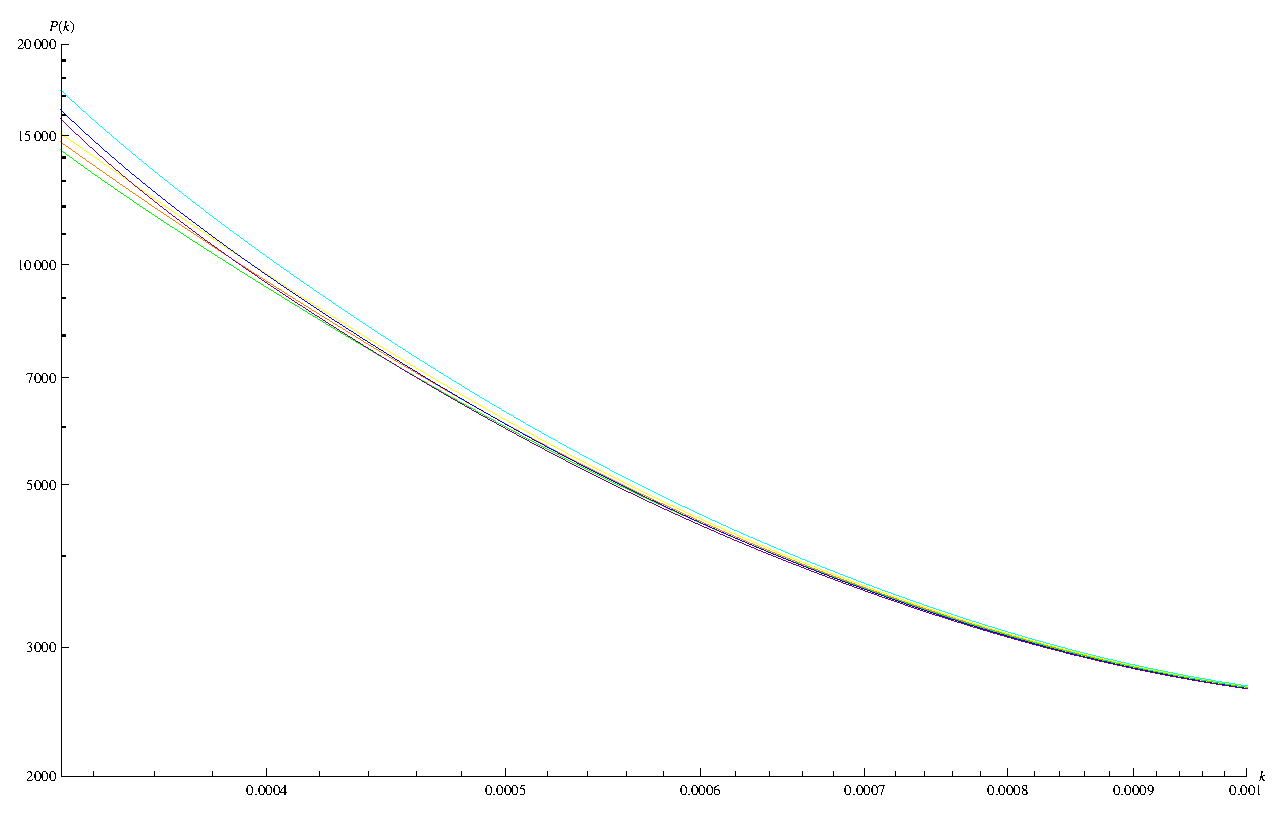
\includegraphics[width=350pt]{CPL_Supp_PowerSpectrums_Detail.eps}
\caption{\color{blue}Power spectrum of CPL dark energy and LCDM in units of sCDM.}\label{fig:CPL_Supp_PowerSpectrums_Detail}
\end{figure}

The parameters chosen only have effects on small redshift. This is because the parameters all satisfy the condition that $w_0\rightarrow -1$ and $w_a\rightarrow 0$.

By comparing yellow line ($w_0=-1, w_a=0.1$) and green line ($w_0=-1, w_a=-0.1$), we can see positive $w_a$ leads to a larger then LCDM Hubble distance when $w_0=-1$. This is in accord with the series form of Hubble equation \ref{eq:CPL_HubbleEquation_Series} since $w_0=-1$ eliminates the first order term and the $w_a$ determines whether the expression is larger then one.
Other comparisons like green line and blue line, blue line and purple line in Figure \ref{fig:CPL_Supp_HubbleDistances} \ref{fig:CPL_Supp_HubbleDistances_Cut} \ref{fig:CPL_Supp_HubbleDistances_DivideLCDM} can also be interpreted by equation \ref{eq:CPL_HubbleEquation_Series}.


Growth factors are also following the expansion. Cyan line ($w_0=-0.9, w_a=0.1$) has smaller Hubble distances that others at late time, so the growth drops since growth factor is positively correlated to the size of the Hubble distance. The changes in growth factors when changing the parameters are exactly positively correlated to the size of Hubble distance changes. For example, the yellow line ($w_0=-1, w_a=0.1$) crosses the purple line ($w_0=-0.9, w_a=-0.2$) in figure \ref{fig:CPL_Supp_GrowthFactors} \ref{fig:CPL_Supp_GrowthFactors_Cut} as they cross each other in the figure of Hubble distance.

Figure \ref{fig:CPL_Supp_QFactors} has a region $k<3.3 * 10^{-4}$ that is corresponding to scale factor $a>1$. So I give another two plots figure \ref{fig:CPL_Supp_QFactors_Cut} and \ref{fig:CPL_Supp_QFactors_Detail}. The same thing is done for power spectrum.

The power spectrum is consistent with the Hubble distance figure: larger Hubble distance generates weaker power.




\item
Because we are using adiabatic initial conditions with a form $P\sim \frac{1}{k^3}$.

At $a\sim 10^{-3}$ and $a\sim 1$, we have $k\sim 1$ and $k\sim 10^{-3}$ correspondingly. The growth factor with amplifies the initial perturbation by about $10^3$ to get the current value $P\sim 10^6$ for $k\sim 1$ and the current value is $10^9$ for initial perturbation at $a\sim 1$ (or $k\sim 10^{-3}$) since it has not evolved. This simple calculation show the shape of power spectrum is definitely going up at small k.

item
As stated previously, the inconsistent part is $z<0$, so there is no need to worry about.





\end{enumerate}



}
\end{quotation}





\section{Appendix}

\subsection{Growth Factor Revisited}

In this part, prime (') stands for the derivative with time $t$, over dot stands for the derivative with scale factor $a$.

Use Navier Stokes equations for matter (with pressure $p=0$) as the basic equation set. {\footnote{{\it Cosmology Project} Notebook}}

Using $\delta_m=\frac{\rho_m-\bar\rho_m}{\bar\rho_m}$, the equations become
\begin{eqnarray}
\frac{\partial {\delta_m}}{\partial t}+a^{-1}\vec{v}_m\cdot \delta_m &=& -a^{-1}(1+\delta_m)\nabla\cdot\vec{v}_m \\
\frac{\partial \vec{v}_m}{\partial t}+ a^{-1}(\vec{v}_m\cdot \nabla)\vec v_m &=& -\frac{\nabla\Phi}{a}-H\vec v_m \\
a^{-2}\nabla^2\Phi &=& 4\pi G\bar\rho_m\delta_m
\end{eqnarray}

In these equations, $\Phi$ is the gravitational potential.

This is too complex to solve. So we only use the linear approximation,that is, no second or higher order of $\delta_m$, $\vec v_m$, $\Phi$ appear, because we already use those as perturbations.
Finally,
\begin{eqnarray}
\frac{\partial {\delta_m}}{\partial t}&=&-a^{-1}\nabla \cdot\vec{v}_m \\
\frac{\partial \vec{v}_m}{\partial t}&=& -\frac{\nabla\Phi}{a}-H\vec v_m \\
a^{-2}\nabla^2\Phi &=& 4\pi G\bar\rho_m\delta_m
\end{eqnarray}

Easily, one can use the well known trick for this kind of equations to find the second derivative equation for $\delta_m$, or the basic function for this problem,
\begin{eqnarray}
\delta_{m}''+2H\delta_m'-4\pi G \bar\rho_m \delta_m=0
\end{eqnarray}

However, we usually use scale factor $a$ as a measurement of time. Thus we would transform it the following form
\begin{equation}
\ddot \delta_m+(\frac{\mathrm d\ln{H}}{\mathrm da}+\frac{3}{a})-\frac{3\Omega_{m0}H_0^2}{2a^5H^2}\delta_m =0
\end{equation}

Almost each book of ODE will tell us how to solve such an equation.

After a little work, we will get two special solutions:
\begin{eqnarray}
\delta_{m,1}&=&H \\
\delta_{m,2}&=&H\int^a_0 \frac1{a'^3H(a')^3}\mathrm d a'
\end{eqnarray}

General solution is
\begin{equation}
\delta_m=C_1 H+C H\int^a_0 \frac{1}{a'^3H(a')^3}\mathrm da'
\end{equation}

Since $H$ is decaying, drop $C_1 H$, then
\begin{equation}
\delta_m=C H\int^a_0 \frac{1}{a'^3H(a')^3}\mathrm da'
\end{equation}

Apply initial condition $\delta_m(a_{i})=\delta_{i}$
\begin{equation}
C=\frac{\delta_i}{H(a_i)}\frac{1}{\int^{a_i}_0\frac{1}{a'^3H(a')^3}}\mathrm d a'
\end{equation}

To simplify these expressions, we now define $D_+=\frac 5 2 \Omega_{m0} H(a) \int^a_0\frac{1}{a'^3H(a')^3}\mathrm d a'$. (One might be confused with this defination at first. The constant multiplied the the original part is to ensure one condition: at matter domination,$D_+$ is $a$. This condition endow $D_+$ with more physics.) Then 
\begin{equation}
C=\delta_i \frac {5\Omega_{m0}H_0^2}{2} \frac1{D_+(a_i)}
\end{equation}

With this, we have
\begin{equation}
\delta_m(a)=\delta_i \frac{D_+(a)}{D_+(a_i)}
\end{equation}

Actually, this $D_+(a)$ is a growing mode of the equation, and we all call it growth factor.




\subsection{CPL}

\subsubsection{Equation of State}

\begin{equation}
w(a)=w_0+w_a(1-a)=w_0+w_a\frac{z}{1+z}
\end{equation}


\subsubsection{Hubble Function}

By solving the Friedmann equation using the CPL parameterisation, the contribution to the background of CPL dark energy is $\Omega_{de0}a^{-3(1+w_0+w_a)}e^{-3w_a(1-a)}$.

Thus the Hubble function should be
\begin{equation}
H(a)=H_0\sqrt{\Omega_{m0}a^{-3}+\Omega_{r0}a^{-4}+\Omega_{de0}a^{-3(1+w_0+w_a)}e^{-3w_a(1-a)}}
\end{equation}


The Taylor series of dark energy contribution is
\begin{equation}
a^{-3(1+w_a+w_0)}e^{-3w_a(1-a)}=1+3(1+w_0)(a-1)+\frac 3 2 (4+w_a+7w_0+3w_0^2)(1-a)^2+...\label{eq:CPL_HubbleEquation_Series}
\end{equation}

To create a mimic of LCDM at low redshift, $w_0\rightarrow 0$ should be satisfied. To make a more rigorous condition, $w_a$ should be much smaller than 1 for this cancels the contribution of $z^2$ term once $w_0=-1$.


In order to generate a background similar to LCDM, the parameters should carefully chosen according to the criteria that $w_0\rightarrow 0$ and $w_a\rightarrow 0$.
















%Actually, this subsection "Supplements2" is a part of chapter "Work". After this is finished, add it to "Work".

\begin{quotation}
{\color{JungleGreen}
\subsection{Second Supplements}


\subsubsection{To Think More}

\begin{enumerate}

\item
A little dimensional analysis is shown here, in case of future mistakes.
\begin{enumerate}
\item
Hubble constant, $H_0$ carries the dimension of $[Time]^{-1}$
\item
Gravitational constant, $G$ carries the dimension of $[Length]^3/[Mass][Time]^2$
\item
Speed of light in vacuum, $c$ of course, has the dimension of $[Length]/[Time]$

\end{enumerate}


\item
Large $k$ corresponds to the future. Besides, large $k$ should have the same amplitude because they have not come inside the horizon.

\item
What's more, the comoving horizon becomes constant in the far future.

\begin{figure}[!htpb]
\centering
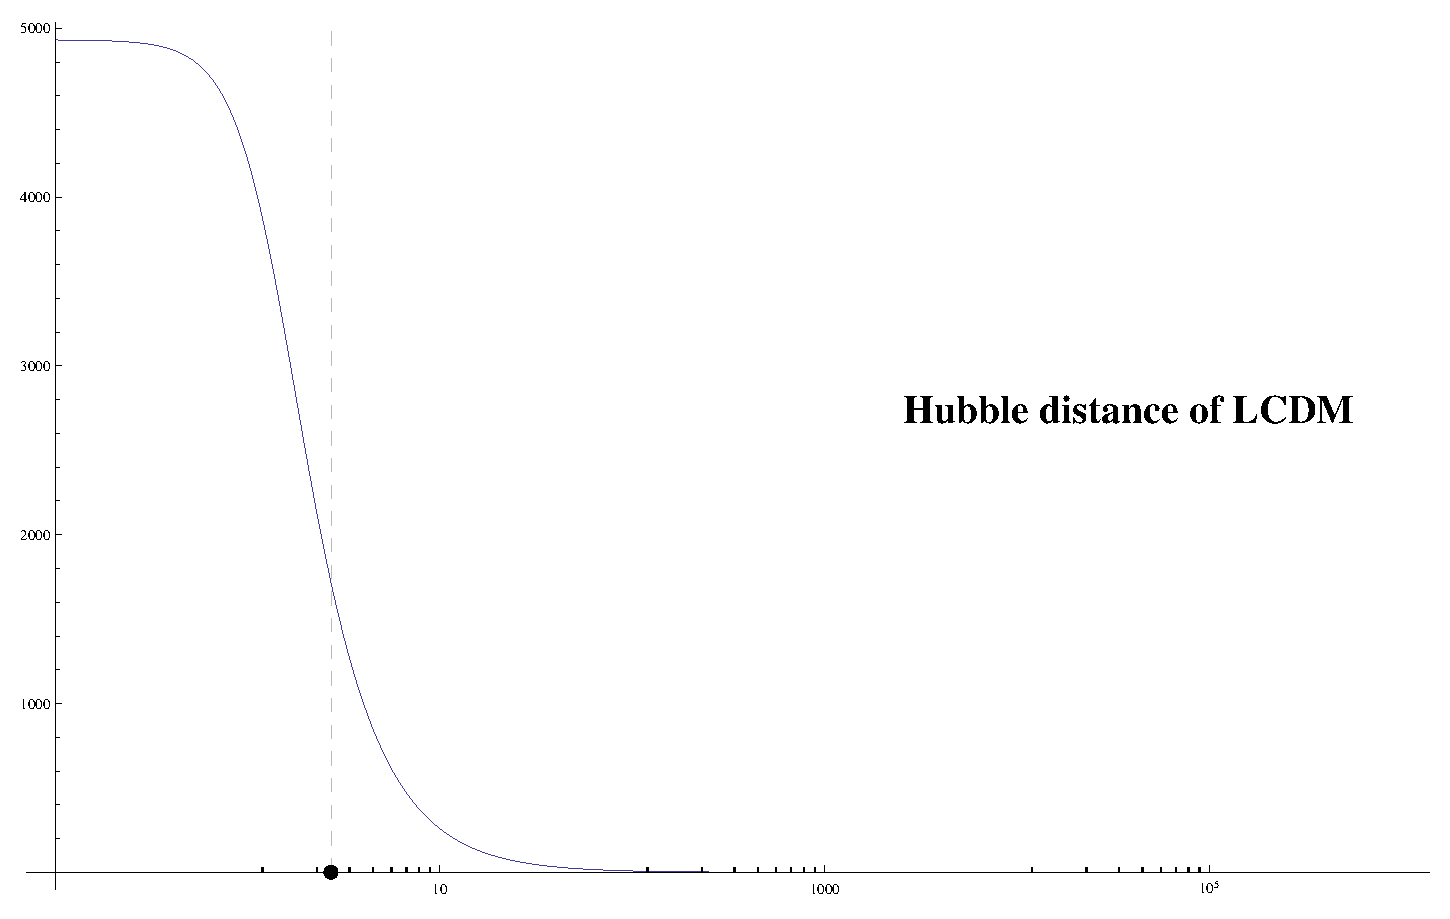
\includegraphics[width=350pt]{HubbleDistanceOfLCDM_Marked.eps}
\caption{\color{JungleGreen}Hubble distance of LCDM model. The dashed vertical line is zero redshift.}\label{fig:DE_Supp_HubbleDistances}
\end{figure}

This simply means there are perturbations that will never come into the horizon.

To calculate the power spectrum, one should cut the growth functions at $z=0$ and set the matter perturbation the same then calculate on. Since these are outside of the horizon, today's power spectrum seems weird.

\item
The power spectrum calculated by me is the power of today. However, observations certainly won't get the power spectrum of the present day. On large scales, the distribution of matter is the in the state of earlier ages.

In paper {\bf Matter power spectrum from the Lyman-alpha forest: myth or reality?} ({\it Mon. Not. R. Astron. Soc. 334, 107-116, 2002}) calculated the distribution of matter at $z=2.72$. This paper also assumed that the underlying baryon density follows that of dark matter (their reference is Croft et al, 2001, astro-ph/0012324).





\end{enumerate}











}
\end{quotation}









\subsection{Including DM-DE perturbation}






























\section{Todo List}
\begin{itemize}
\item
\sout{Find all the growth factors if they are useful.}
\item
\sout{Calculate the fiducial power spectrum.}

\item
\sout{The spectrum is normalised to be the same at $a\sim 0$. So that the $\sigma_8$ of different models are the same.}

\item
Switch from adiabatic initial condition to isocurvature initial condition will change the expression of growth factors (changing the power of H), thus leading to different results.

\item
Introduce interacting between dark energy and dark matter.

\item
Other quantities in cosmology? Can one generalise this method to more calculations?


\end{itemize}















\section{Appendix}

\subsection{Growth Factor Revisited}

In this part, prime (') stands for the derivative with time $t$, over dot stands for the derivative with scale factor $a$.

Use Navier Stokes equations for matter (with pressure $p=0$) as the basic equation set. {\footnote{{\it Cosmology Project} Notebook}}

Using $\delta_m=\frac{\rho_m-\bar\rho_m}{\bar\rho_m}$, the equations become
\begin{eqnarray}
\frac{\partial {\delta_m}}{\partial t}+a^{-1}\vec{v}_m\cdot \delta_m &=& -a^{-1}(1+\delta_m)\nabla\cdot\vec{v}_m \\
\frac{\partial \vec{v}_m}{\partial t}+ a^{-1}(\vec{v}_m\cdot \nabla)\vec v_m &=& -\frac{\nabla\Phi}{a}-H\vec v_m \\
a^{-2}\nabla^2\Phi &=& 4\pi G\bar\rho_m\delta_m
\end{eqnarray}

In these equations, $\Phi$ is the gravitational potential.

This is too complex to solve. So we only use the linear approximation,that is, no second or higher order of $\delta_m$, $\vec v_m$, $\Phi$ appear, because we already use those as perturbations.
Finally,
\begin{eqnarray}
\frac{\partial {\delta_m}}{\partial t}&=&-a^{-1}\nabla \cdot\vec{v}_m \\
\frac{\partial \vec{v}_m}{\partial t}&=& -\frac{\nabla\Phi}{a}-H\vec v_m \\
a^{-2}\nabla^2\Phi &=& 4\pi G\bar\rho_m\delta_m
\end{eqnarray}

Easily, one can use the well known trick for this kind of equations to find the second derivative equation for $\delta_m$, or the basic function for this problem,
\begin{eqnarray}
\delta_{m}''+2H\delta_m'-4\pi G \bar\rho_m \delta_m=0
\end{eqnarray}

However, we usually use scale factor $a$ as a measurement of time. Thus we would transform it the following form
\begin{equation}
\ddot \delta_m+(\frac{\mathrm d\ln{H}}{\mathrm da}+\frac{3}{a})-\frac{3\Omega_{m0}H_0^2}{2a^5H^2}\delta_m =0
\end{equation}

Almost each book of ODE will tell us how to solve such an equation.

After a little work, we will get two special solutions:
\begin{eqnarray}
\delta_{m,1}&=&H \\
\delta_{m,2}&=&H\int^a_0 \frac1{a'^3H(a')^3}\mathrm d a'
\end{eqnarray}

General solution is
\begin{equation}
\delta_m=C_1 H+C H\int^a_0 \frac{1}{a'^3H(a')^3}\mathrm da'
\end{equation}

Since $H$ is decaying, drop $C_1 H$, then
\begin{equation}
\delta_m=C H\int^a_0 \frac{1}{a'^3H(a')^3}\mathrm da'
\end{equation}

Apply initial condition $\delta_m(a_{i})=\delta_{i}$
\begin{equation}
C=\frac{\delta_i}{H(a_i)}\frac{1}{\int^{a_i}_0\frac{1}{a'^3H(a')^3}}\mathrm d a'
\end{equation}

To simplify these expressions, we now define $D_+=\frac 5 2 \Omega_{m0} H(a) \int^a_0\frac{1}{a'^3H(a')^3}\mathrm d a'$. (One might be confused with this defination at first. The constant multiplied the the original part is to ensure one condition: at matter domination,$D_+$ is $a$. This condition endow $D_+$ with more physics.) Then 
\begin{equation}
C=\delta_i \frac {5\Omega_{m0}H_0^2}{2} \frac1{D_+(a_i)}
\end{equation}

With this, we have
\begin{equation}
\delta_m(a)=\delta_i \frac{D_+(a)}{D_+(a_i)}
\end{equation}

Actually, this $D_+(a)$ is a growing mode of the equation, and we all call it growth factor.




\subsection{CPL}

\subsubsection{Equation of State}

\begin{equation}
w(a)=w_0+w_a(1-a)=w_0+w_a\frac{z}{1+z}
\end{equation}


\subsubsection{Hubble Function}

By solving the Friedmann equation using the CPL parameterisation, the contribution to the background of CPL dark energy is $\Omega_{de0}a^{-3(1+w_0+w_a)}e^{-3w_a(1-a)}$.

Thus the Hubble function should be
\begin{equation}
H(a)=H_0\sqrt{\Omega_{m0}a^{-3}+\Omega_{r0}a^{-4}+\Omega_{de0}a^{-3(1+w_0+w_a)}e^{-3w_a(1-a)}}
\end{equation}


The Taylor series of dark energy contribution is
\begin{equation}
a^{-3(1+w_a+w_0)}e^{-3w_a(1-a)}=1+3(1+w_0)(a-1)+\frac 3 2 (4+w_a+7w_0+3w_0^2)(1-a)^2+...\label{eq:CPL_HubbleEquation_Series}
\end{equation}

To create a mimic of LCDM at low redshift, $w_0\rightarrow 0$ should be satisfied. To make a more rigorous condition, $w_a$ should be much smaller than 1 for this cancels the contribution of $z^2$ term once $w_0=-1$.


In order to generate a background similar to LCDM, the parameters should carefully chosen according to the criteria that $w_0\rightarrow 0$ and $w_a\rightarrow 0$.







\end{document}
